\usepackage[a4paper,top=25mm,bottom=24mm,left=27mm,right=23mm,headheight=15pt]{geometry}
\usepackage{fontspec}
\setmainfont{Times New Roman}
\setsansfont{Times New Roman}
\setmonofont{Times New Roman}
\usepackage{amsmath,amssymb,graphicx,booktabs,array,longtable,float,tabularx}
\usepackage{unicode-math}
\setmathfont{Cambria Math}
\usepackage{indentfirst}
\usepackage[table]{xcolor}
\usepackage{enumitem,fancyhdr,titlesec,caption,subcaption,tcolorbox,needspace}
\usepackage{tikz}
\usetikzlibrary{arrows.meta,positioning,calc,fit,backgrounds}
\usepackage[numbers,sort&compress]{natbib}
\usepackage{hyperref}
\hypersetup{colorlinks=true,linkcolor=black,citecolor=black,urlcolor=black,
 pdftitle={CO5085: E1--E3, A1 and A2},pdfauthor={Dang Nguyen Tan Tai}}
\setlength{\parindent}{1cm}
\setlength{\parskip}{4pt}
\linespread{1.1}
\emergencystretch=4em
\raggedbottom
\pagestyle{fancy}
\fancyhf{}
\fancyhead[L]{\small CO5085: E1--E3, A1 và A2}
\fancyhead[R]{\small Học sâu và thị giác máy tính}
\fancyfoot[C]{\thepage}
\renewcommand{\headrulewidth}{0.4pt}
\fancypagestyle{plain}{\fancyhf{}\fancyfoot[C]{\thepage}\renewcommand{\headrulewidth}{0pt}}
\titleformat{\chapter}[hang]{\normalfont\LARGE\bfseries}{\thechapter.}{0.6em}{}
\titlespacing{\chapter}{0pt}{-8pt}{18pt}
\captionsetup{font=small,labelfont=bf}
\renewcommand{\contentsname}{Mục lục}
\renewcommand{\listfigurename}{Danh sách hình vẽ}
\renewcommand{\listtablename}{Danh sách bảng}
\renewcommand{\figurename}{Hình}
\renewcommand{\tablename}{Bảng}
\renewcommand{\bibname}{Tài liệu tham khảo}
\renewcommand{\appendixname}{Phụ lục}
\setlist[itemize]{topsep=3pt,itemsep=2pt,leftmargin=1.6em}
\tikzset{box/.style={draw=black,align=center,
 minimum height=12mm,text width=29mm,font=\small,fill=white},
 fc/.style={box},output/.style={box},
 flow/.style={-{Latex[length=2mm]},thick},
 note/.style={align=center,font=\footnotesize,text width=35mm}}
\newcommand{\ReportFigure}[3][.97]{\begin{figure}[H]\centering
\includegraphics[width=#1\linewidth,keepaspectratio]{#2}\caption{#3}\label{fig:#2}\end{figure}}
\newcommand{\DataTable}[2]{\begin{table}[H]\centering\caption{#2}
\small\setlength{\tabcolsep}{4pt}\input{#1}\label{tab:#1}\end{table}}
\newcommand{\Evidence}[1]{\begin{tcolorbox}[colback=white,colframe=black,
 boxrule=.5pt,arc=1mm]#1\end{tcolorbox}}
% Architecture diagrams use black ink and white fill.
% Tensor faces show spatial dimensions and channel depth.
% All arrows are strictly orthogonal (horizontal, vertical, or right-angle turns).
% Minimal text inside nodes (symbolic), with full explanations in bottom badges.
\usetikzlibrary{arrows.meta,positioning,calc,fit,backgrounds,shapes.geometric,decorations.pathreplacing}

\tikzset{
  % Common styles
  arch_box/.style={draw=black, fill=white, line width=0.6pt, rounded corners=1.5pt, align=center, font=\footnotesize},
  arch_box_gray/.style={draw=black, fill=white, line width=0.6pt, rounded corners=1.5pt, align=center, font=\footnotesize},
  arch_box_dark/.style={draw=black, fill=white, line width=0.6pt, rounded corners=1.5pt, align=center, font=\footnotesize},
  arch_op/.style={draw=black, fill=white, circle, line width=0.6pt, inner sep=1pt, minimum size=5.0mm, font=\small},
  arch_arrow/.style={-{Latex[length=2.2mm,width=1.4mm]}, line width=0.65pt},
  arch_arrow_thick/.style={-{Latex[length=2.5mm,width=1.6mm]}, line width=0.85pt},
  arch_line/.style={draw=black, line width=0.65pt},
  arch_dash/.style={draw=black, dashed, line width=0.6pt},
  arch_label/.style={font=\footnotesize, align=center, fill=white, inner sep=1.5pt},
  arch_title/.style={font=\small\bfseries, align=center},
  arch_badge/.style={draw=black, fill=white, rounded corners=1mm, font=\scriptsize, align=center, inner sep=2.5pt}
}

% -------------------------------------------------------------
% Helper: 2.5D Isometric Tensor Drawing
% #1: name
% #2: x
% #3: y (bottom of front face)
% #4: width (front face x-dim)
% #5: height (front face y-dim)
% #6: depth (isometric projection length)
% #7: line width (pt)
% #8: label below (optional)
% -------------------------------------------------------------
\newcommand{\TensorMap}[8]{%
\begin{scope}[shift={(#2,#3)}]
\pgfmathsetmacro{\dx}{#6*0.707}
\pgfmathsetmacro{\dy}{#6*0.5}
% Top face
\draw[draw=black,fill=white,line width=#7pt]
 (0,#5)--(\dx,{#5+\dy})--({#4+\dx},{#5+\dy})--(#4,#5)--cycle;
% Right face
\draw[draw=black,fill=white,line width=#7pt]
 (#4,0)--({#4+\dx},\dy)--({#4+\dx},{#5+\dy})--(#4,#5)--cycle;
% Channel slices on right face if depth is noticeable
\ifdim #6pt>0.25pt
  \foreach \q in {0.33, 0.66}{
    \draw[black,line width=0.35pt]
     ({#4+\dx*\q},{\dy*\q})--({#4+\dx*\q},{#5+\dy*\q});
  }
\fi
% Front face
\draw[draw=black,fill=white,line width=#7pt] (0,0) rectangle (#4,#5);
% Standard anchors
\coordinate (#1-west) at (0,{#5/2});
\coordinate (#1-east) at ({#4+\dx},{#5/2+\dy/2});
\coordinate (#1-front-east) at (#4,{#5/2});
\coordinate (#1-north) at ({#4/2+\dx/2},{#5+\dy});
\coordinate (#1-south) at ({#4/2},0);
\coordinate (#1-center) at ({#4/2+\dx/2},{#5/2+\dy/2});
\if\relax\detokenize{#8}\relax\else
  \node[font=\footnotesize,align=center,anchor=north,inner sep=2pt] at ({#4/2}, -0.15) {#8};
\fi
\end{scope}}

% =============================================================
% 1. ARCHITECTURE: Softmax Classifier
% =============================================================
\newcommand{\ArchSoftmax}{%
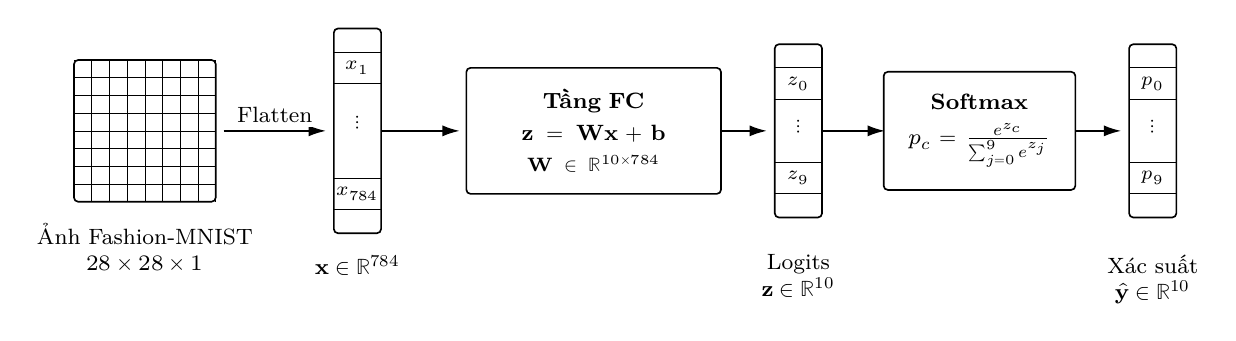
\begin{tikzpicture}[x=1cm,y=1cm]
  % Input image
  \node[arch_box, minimum width=1.8cm, minimum height=1.8cm, fill=white] (im) at (0, 0) {};
  \draw[step=0.225cm, black, line width=0.25pt] (-0.9,-0.9) grid (0.9,0.9);
  \node[font=\footnotesize, anchor=north, align=center] at (0, -1.05) {Ảnh Fashion-MNIST\\$28\times 28\times 1$};

  % Flatten arrow
  \draw[arch_arrow] (1.0, 0) -- node[above=1pt, font=\footnotesize, fill=white, inner sep=1.5pt] {Flatten} (2.3, 0);

  % 1D Vector
  \node[arch_box, minimum width=0.6cm, minimum height=2.6cm, fill=white] (vec) at (2.7, 0) {};
  \foreach \y in {-1.0, -0.6, 0.6, 1.0}{ \draw[black, line width=0.3pt] (2.4, \y) -- (3.0, \y); }
  \node[font=\scriptsize] at (2.7, 0.8) {$x_1$};
  \node[font=\scriptsize] at (2.7, 0.1) {$\vdots$};
  \node[font=\scriptsize] at (2.7, -0.8) {$x_{784}$};
  \node[font=\footnotesize, anchor=north, align=center] at (2.7, -1.45) {$\mathbf{x} \in \mathbb{R}^{784}$};

  % Linear transformation block
  \draw[arch_arrow] (vec.east) -- (4.0, 0);
  \node[arch_box_gray, text width=3.0cm, minimum height=1.6cm] (fc) at (5.7, 0) {
    \textbf{Tầng FC}\\[2pt]
    $\mathbf{z} = \mathbf{W}\mathbf{x} + \mathbf{b}$\\[2pt]
    \scriptsize $\mathbf{W} \in \mathbb{R}^{10\times 784}$
  };

  % Logits vector
  \draw[arch_arrow] (fc.east) -- (7.9, 0);
  \node[arch_box, minimum width=0.6cm, minimum height=2.2cm, fill=white] (logits) at (8.3, 0) {};
  \foreach \y in {-0.8, -0.4, 0.4, 0.8}{ \draw[black, line width=0.3pt] (8.0, \y) -- (8.6, \y); }
  \node[font=\scriptsize] at (8.3, 0.6) {$z_0$};
  \node[font=\scriptsize] at (8.3, 0.05) {$\vdots$};
  \node[font=\scriptsize] at (8.3, -0.6) {$z_9$};
  \node[font=\footnotesize, anchor=north, align=center] at (8.3, -1.45) {Logits\\$\mathbf{z} \in \mathbb{R}^{10}$};

  % Softmax block
  \draw[arch_arrow] (logits.east) -- (9.4, 0);
  \node[arch_box_dark, text width=2.2cm, minimum height=1.5cm] (sm) at (10.6, 0) {
    \textbf{Softmax}\\[3pt]
    $p_c = \frac{e^{z_c}}{\sum_{j=0}^{9} e^{z_j}}$
  };

  % Output probabilities
  \draw[arch_arrow] (sm.east) -- (12.4, 0);
  \node[arch_box, minimum width=0.6cm, minimum height=2.2cm, fill=white] (prob) at (12.8, 0) {};
  \foreach \y in {-0.8, -0.4, 0.4, 0.8}{ \draw[black, line width=0.3pt] (12.5, \y) -- (13.1, \y); }
  \node[font=\scriptsize] at (12.8, 0.6) {$p_0$};
  \node[font=\scriptsize] at (12.8, 0.05) {$\vdots$};
  \node[font=\scriptsize] at (12.8, -0.6) {$p_9$};
  \node[font=\footnotesize, anchor=north, align=center] at (12.8, -1.45) {Xác suất\\$\hat{\mathbf{y}} \in \mathbb{R}^{10}$};

  % Note / equation at bottom dự đoán nhãn bằng $\hat{y} = \operatorname{argmax}_c z_c$, tổng $7,850$ tham số ($10\times 784$ trọng số + $10$ bias)};
\end{tikzpicture}}

% =============================================================
% 2. ARCHITECTURE: MLP
% =============================================================
\newcommand{\ArchMLP}{%
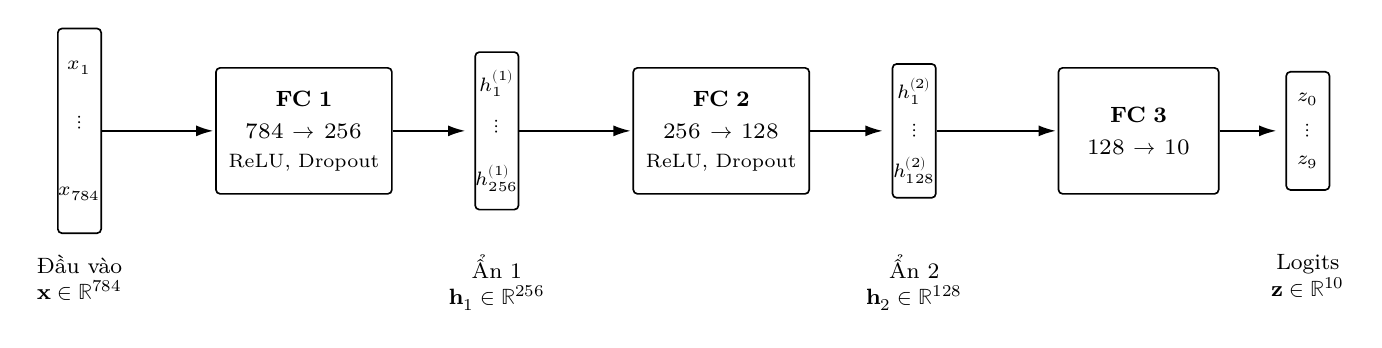
\begin{tikzpicture}[x=1cm,y=1cm]
  % Input vector
  \node[arch_box, minimum width=0.55cm, minimum height=2.6cm, fill=white] (in) at (0, 0) {};
  \node[font=\scriptsize] at (0, 0.8) {$x_1$};
  \node[font=\scriptsize] at (0, 0.1) {$\vdots$};
  \node[font=\scriptsize] at (0, -0.8) {$x_{784}$};
  \node[font=\footnotesize, anchor=north, align=center] at (0, -1.45) {Đầu vào\\$\mathbf{x} \in \mathbb{R}^{784}$};

  % Hidden layer 1
  \draw[arch_arrow] (in.east) -- (1.7, 0);
  \node[arch_box, text width=2.0cm, minimum height=1.6cm, fill=white] (fc1) at (2.85, 0) {
    \textbf{FC 1}\\[2pt]
    $784 \to 256$\\[1pt]
    \scriptsize ReLU, Dropout
  };

  % Feature h1
  \draw[arch_arrow] (fc1.east) -- (4.9, 0);
  \node[arch_box, minimum width=0.55cm, minimum height=2.0cm, fill=white] (h1) at (5.3, 0) {};
  \node[font=\scriptsize] at (5.3, 0.6) {$h_1^{(1)}$};
  \node[font=\scriptsize] at (5.3, 0.05) {$\vdots$};
  \node[font=\scriptsize] at (5.3, -0.6) {$h_{256}^{(1)}$};
  \node[font=\footnotesize, anchor=north, align=center] at (5.3, -1.45) {Ẩn 1\\$\mathbf{h}_1 \in \mathbb{R}^{256}$};

  % Hidden layer 2
  \draw[arch_arrow] (h1.east) -- (7.0, 0);
  \node[arch_box, text width=2.0cm, minimum height=1.6cm, fill=white] (fc2) at (8.15, 0) {
    \textbf{FC 2}\\[2pt]
    $256 \to 128$\\[1pt]
    \scriptsize ReLU, Dropout
  };

  % Feature h2
  \draw[arch_arrow] (fc2.east) -- (10.2, 0);
  \node[arch_box, minimum width=0.55cm, minimum height=1.7cm, fill=white] (h2) at (10.6, 0) {};
  \node[font=\scriptsize] at (10.6, 0.5) {$h_1^{(2)}$};
  \node[font=\scriptsize] at (10.6, 0.0) {$\vdots$};
  \node[font=\scriptsize] at (10.6, -0.5) {$h_{128}^{(2)}$};
  \node[font=\footnotesize, anchor=north, align=center] at (10.6, -1.45) {Ẩn 2\\$\mathbf{h}_2 \in \mathbb{R}^{128}$};

  % Output FC
  \draw[arch_arrow] (h2.east) -- (12.4, 0);
  \node[arch_box, text width=1.8cm, minimum height=1.6cm, fill=white] (fco) at (13.45, 0) {
    \textbf{FC 3}\\[2pt]
    $128 \to 10$
  };

  % Output logits
  \draw[arch_arrow] (fco.east) -- (15.2, 0);
  \node[arch_box, minimum width=0.55cm, minimum height=1.5cm, fill=white] (out) at (15.6, 0) {};
  \node[font=\scriptsize] at (15.6, 0.4) {$z_0$};
  \node[font=\scriptsize] at (15.6, 0.0) {$\vdots$};
  \node[font=\scriptsize] at (15.6, -0.4) {$z_9$};
  \node[font=\footnotesize, anchor=north, align=center] at (15.6, -1.45) {Logits\\$\mathbf{z} \in \mathbb{R}^{10}$};

  % Capacity note tổng $235,146$ tham số học được};
\end{tikzpicture}}

% =============================================================
% 3. ARCHITECTURE: CNN-A
% =============================================================
\newcommand{\ArchCNNA}{%
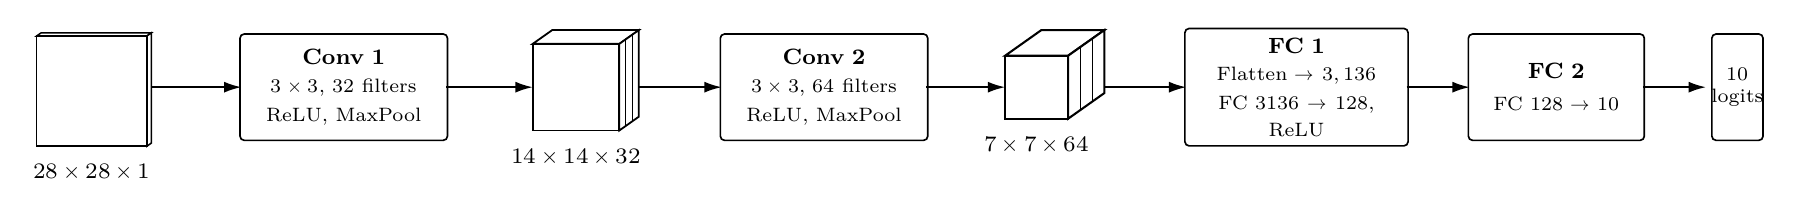
\begin{tikzpicture}[x=1cm,y=1cm]
  \def\cy{0.75}

  % Input map
  \TensorMap{im}{0}{0}{1.4}{1.4}{0.08}{0.55}{$28\times 28\times 1$}

  % Conv 1 operation
  \draw[arch_arrow] (1.45, \cy) -- (2.6, \cy);
  \node[arch_box, text width=2.4cm, minimum height=1.35cm] (op1) at (3.9, \cy) {
    \textbf{Conv 1}\\[2pt]
    \scriptsize $3\times 3$, $32$ filters\\[1pt]
    ReLU, MaxPool
  };

  % Feature map 1
  \draw[arch_arrow] (5.2, \cy) -- (6.3, \cy);
  \TensorMap{fm1}{6.3}{0.2}{1.1}{1.1}{0.35}{0.65}{$14\times 14\times 32$}

  % Conv 2 operation
  \draw[arch_arrow] (7.65, \cy) -- (8.7, \cy);
  \node[arch_box, text width=2.4cm, minimum height=1.35cm] (op2) at (10.0, \cy) {
    \textbf{Conv 2}\\[2pt]
    \scriptsize $3\times 3$, $64$ filters\\[1pt]
    ReLU, MaxPool
  };

  % Feature map 2
  \draw[arch_arrow] (11.3, \cy) -- (12.3, \cy);
  \TensorMap{fm2}{12.3}{0.35}{0.8}{0.8}{0.65}{0.75}{$7\times 7\times 64$}

  % Flatten & FC 1
  \draw[arch_arrow] (13.56, \cy) -- (14.6, \cy);
  \node[arch_box_gray, text width=2.6cm, minimum height=1.35cm] (fc1) at (16.0, \cy) {
    \textbf{FC 1}\\[2pt]
    \scriptsize Flatten $\to 3,136$\\[1pt]
    FC $3136 \to 128$, ReLU
  };

  % FC 2
  \draw[arch_arrow] (17.4, \cy) -- (18.2, \cy);
  \node[arch_box, text width=2.0cm, minimum height=1.35cm] (fc2) at (19.3, \cy) {
    \textbf{FC 2}\\[2pt]
    \scriptsize FC $128 \to 10$
  };

  % Logits
  \draw[arch_arrow] (20.4, \cy) -- (21.2, \cy);
  \node[arch_box_dark, minimum width=0.65cm, minimum height=1.35cm] (out) at (21.6, \cy) {};
  \node[font=\scriptsize, align=center] at (21.6, \cy) {$10$\\logits};

  % Note below tổng $421,642$ tham số};
\end{tikzpicture}}

% =============================================================
% 4. ARCHITECTURE: CNN-B
% =============================================================
\newcommand{\ArchCNNB}{%
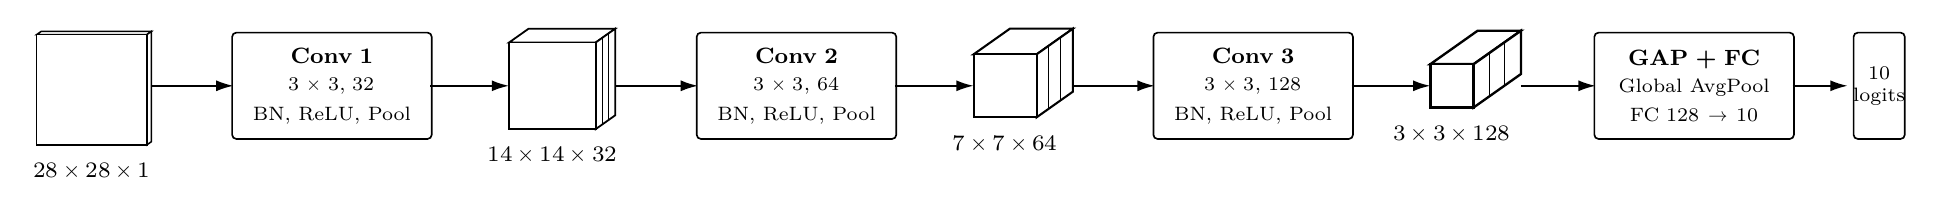
\begin{tikzpicture}[x=1cm,y=1cm]
  \def\cy{0.75}

  % Input map
  \TensorMap{im}{0}{0}{1.4}{1.4}{0.08}{0.55}{$28\times 28\times 1$}

  % Conv 1
  \draw[arch_arrow] (1.45, \cy) -- (2.5, \cy);
  \node[arch_box, text width=2.3cm, minimum height=1.35cm] (op1) at (3.75, \cy) {
    \textbf{Conv 1}\\[2pt]
    \scriptsize $3\times 3$, $32$\\[1pt]
    BN, ReLU, Pool
  };

  % FM1
  \draw[arch_arrow] (5.0, \cy) -- (6.0, \cy);
  \TensorMap{fm1}{6.0}{0.2}{1.1}{1.1}{0.35}{0.65}{$14\times 14\times 32$}

  % Conv 2
  \draw[arch_arrow] (7.35, \cy) -- (8.4, \cy);
  \node[arch_box, text width=2.3cm, minimum height=1.35cm] (op2) at (9.65, \cy) {
    \textbf{Conv 2}\\[2pt]
    \scriptsize $3\times 3$, $64$\\[1pt]
    BN, ReLU, Pool
  };

  % FM2
  \draw[arch_arrow] (10.9, \cy) -- (11.9, \cy);
  \TensorMap{fm2}{11.9}{0.35}{0.8}{0.8}{0.65}{0.75}{$7\times 7\times 64$}

  % Conv 3
  \draw[arch_arrow] (13.16, \cy) -- (14.2, \cy);
  \node[arch_box, text width=2.3cm, minimum height=1.35cm] (op3) at (15.45, \cy) {
    \textbf{Conv 3}\\[2pt]
    \scriptsize $3\times 3$, $128$\\[1pt]
    BN, ReLU, Pool
  };

  % FM3
  \draw[arch_arrow] (16.7, \cy) -- (17.7, \cy);
  \TensorMap{fm3}{17.7}{0.475}{0.55}{0.55}{0.85}{0.85}{$3\times 3\times 128$}

  % GAP & FC head
  \draw[arch_arrow] (18.85, \cy) -- (19.8, \cy);
  \node[arch_box_gray, text width=2.3cm, minimum height=1.35cm] (gap) at (21.05, \cy) {
    \textbf{GAP + FC}\\[2pt]
    \scriptsize Global AvgPool\\[1pt]
    FC $128 \to 10$
  };

  % Out
  \draw[arch_arrow] (22.3, \cy) -- (23.0, \cy);
  \node[arch_box_dark, minimum width=0.65cm, minimum height=1.35cm] (out) at (23.4, \cy) {};
  \node[font=\scriptsize, align=center] at (23.4, \cy) {$10$\\logits};

  % Note below tổng $94,186$ tham số (giảm $4{,}48$ lần)};
\end{tikzpicture}}

% =============================================================
% 5. ARCHITECTURE: Tokenizers
% =============================================================
\newcommand{\ArchTokens}{%
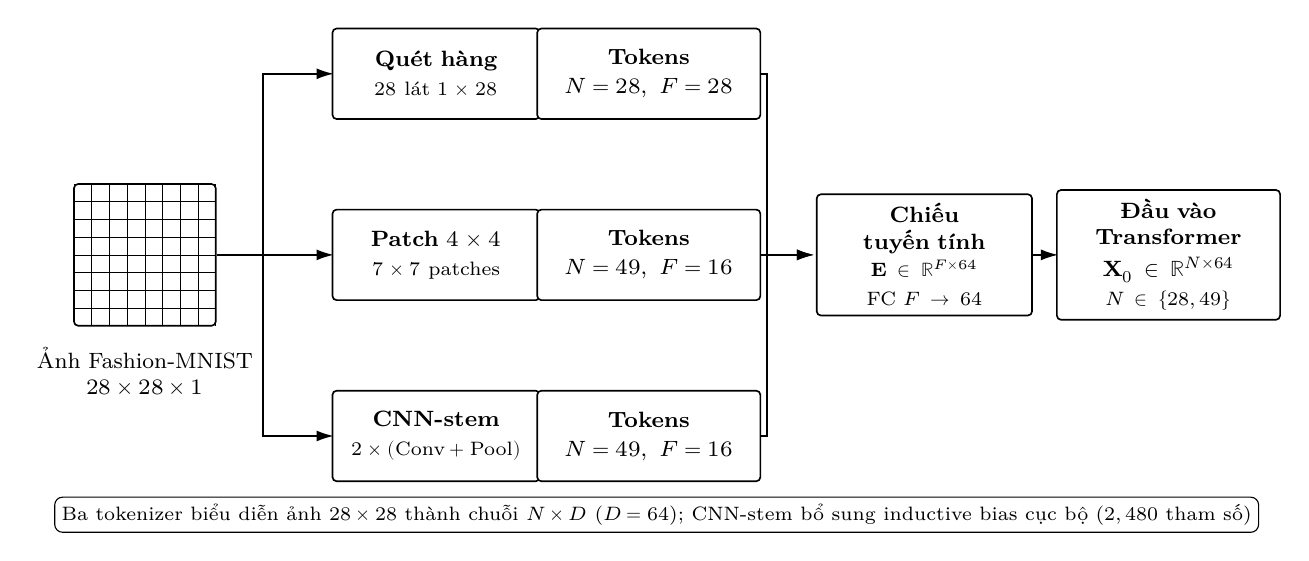
\begin{tikzpicture}[x=1cm,y=1cm]
  % Input image
  \node[arch_box, minimum width=1.8cm, minimum height=1.8cm, fill=white] (im) at (0, 0) {};
  \draw[step=0.225cm, black, line width=0.25pt] (-0.9,-0.9) grid (0.9,0.9);
  \node[font=\footnotesize, anchor=north, align=center] at (0, -1.05) {Ảnh Fashion-MNIST\\$28\times 28\times 1$};

  % Fork (strictly horizontal and vertical)
  \draw[arch_line] (im.east) -- (1.5, 0);
  \draw[arch_arrow] (1.5, 0) |- (2.4, 2.3);
  \draw[arch_arrow] (1.5, 0) -- (2.4, 0);
  \draw[arch_arrow] (1.5, 0) |- (2.4, -2.3);

  % Rows branch
  \node[arch_box, text width=2.4cm, minimum height=1.15cm] (r_desc) at (3.7, 2.3) {
    \textbf{Quét hàng}\\[1pt]
    \scriptsize $28$ lát $1\times 28$
  };
  \draw[arch_arrow] (r_desc.east) -- (5.0, 2.3);
  \node[arch_box_gray, text width=2.6cm, minimum height=1.15cm] (r_tok) at (6.4, 2.3) {
    \textbf{Tokens}\\[1pt]
    \mbox{$N=28,\ F=28$}
  };

  % Patch branch
  \node[arch_box, text width=2.4cm, minimum height=1.15cm] (p_desc) at (3.7, 0) {
    \textbf{Patch $4\times 4$}\\[1pt]
    \scriptsize $7\times 7$ patches
  };
  \draw[arch_arrow] (p_desc.east) -- (5.0, 0);
  \node[arch_box_gray, text width=2.6cm, minimum height=1.15cm] (p_tok) at (6.4, 0) {
    \textbf{Tokens}\\[1pt]
    \mbox{$N=49,\ F=16$}
  };

  % Stem branch
  \node[arch_box, text width=2.4cm, minimum height=1.15cm] (s_desc) at (3.7, -2.3) {
    \textbf{CNN-stem}\\[1pt]
    \scriptsize $2\times (\text{Conv} + \text{Pool})$
  };
  \draw[arch_arrow] (s_desc.east) -- (5.0, -2.3);
  \node[arch_box_gray, text width=2.6cm, minimum height=1.15cm] (s_tok) at (6.4, -2.3) {
    \textbf{Tokens}\\[1pt]
    \mbox{$N=49,\ F=16$}
  };

  % Linear projection block
  \draw[arch_line] (r_tok.east) -- (7.9, 2.3) -- (7.9, 0);
  \draw[arch_arrow] (7.9, 0) -- (8.5, 0);
  \draw[arch_arrow] (p_tok.east) -- (8.5, 0);
  \draw[arch_line] (s_tok.east) -- (7.9, -2.3) -- (7.9, 0);

  \node[arch_box, text width=2.5cm, minimum height=1.45cm] (proj) at (9.9, 0) {
    \textbf{Chiếu tuyến tính}\\[2pt]
    \scriptsize $\mathbf{E} \in \mathbb{R}^{F \times 64}$\\[1pt]
    FC $F \to 64$
  };

  % Tokens out
  \draw[arch_arrow] (proj.east) -- (11.6, 0);
  \node[arch_box_dark, text width=2.6cm, minimum height=1.45cm] (out) at (13.0, 0) {
    \textbf{Đầu vào Transformer}\\[2pt]
    $\mathbf{X}_0 \in \mathbb{R}^{N\times 64}$\\[1pt]
    \scriptsize $N \in \{28, 49\}$
  };

  % Note below
  \node[arch_badge] at (6.5, -3.3) {Ba tokenizer biểu diễn ảnh $28\times 28$ thành chuỗi $N\times D$ ($D=64$); CNN-stem bổ sung inductive bias cục bộ ($2,480$ tham số)};
\end{tikzpicture}}

% =============================================================
% 6. ARCHITECTURE: Transformer Classifier
% =============================================================
\newcommand{\ArchEncoder}{%
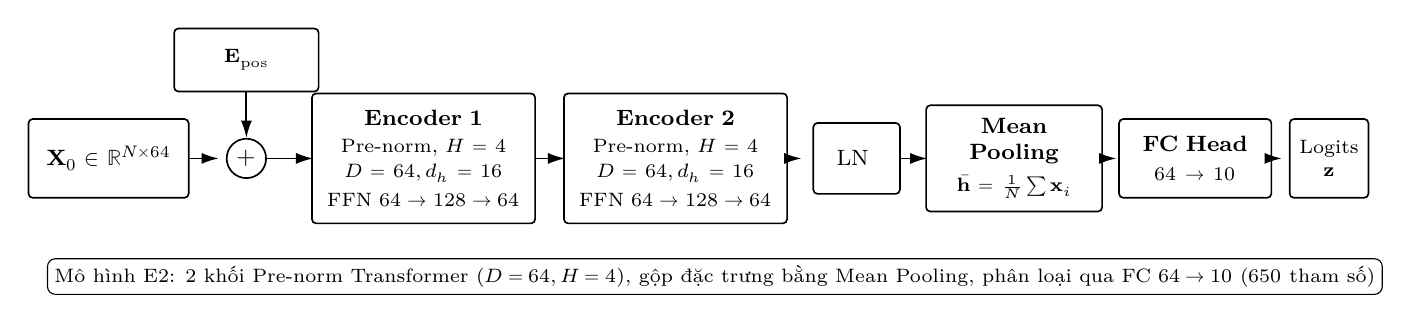
\begin{tikzpicture}[x=1cm,y=1cm]
  % Input tokens
  \node[arch_box, text width=1.8cm, minimum height=1.0cm] (tok) at (0, 0) {
    $\mathbf{X}_0 \in \mathbb{R}^{N\times 64}$
  };

  % Position embedding addition
  \draw[arch_arrow] (tok.east) -- (1.4, 0);
  \node[arch_op] (add_pos) at (1.75, 0) {$+$};

  \node[arch_box, text width=1.6cm, minimum height=0.8cm] (pos) at (1.75, 1.25) {
    \scriptsize $\mathbf{E}_{\mathrm{pos}}$
  };
  \draw[arch_arrow] (pos.south) -- (add_pos.north);

  % Encoder Block 1
  \draw[arch_arrow] (add_pos.east) -- (2.6, 0);
  \node[arch_box_gray, text width=2.6cm, minimum height=1.65cm] (b1) at (4.0, 0) {
    \textbf{Encoder 1}\\[2pt]
    \scriptsize Pre-norm, $H=4$\\[1pt]
    $D=64, d_h=16$\\[1pt]
    FFN $64\to 128\to 64$
  };

  % Encoder Block 2
  \draw[arch_arrow] (b1.east) -- (5.8, 0);
  \node[arch_box_gray, text width=2.6cm, minimum height=1.65cm] (b2) at (7.2, 0) {
    \textbf{Encoder 2}\\[2pt]
    \scriptsize Pre-norm, $H=4$\\[1pt]
    $D=64, d_h=16$\\[1pt]
    FFN $64\to 128\to 64$
  };

  % Final LayerNorm
  \draw[arch_arrow] (b2.east) -- (8.8, 0);
  \node[arch_box, minimum width=1.1cm, minimum height=0.9cm] (ln) at (9.5, 0) {
    $\mathrm{LN}$
  };

  % Mean Pooling
  \draw[arch_arrow] (ln.east) -- (10.4, 0);
  \node[arch_box, text width=2.0cm, minimum height=1.35cm] (pool) at (11.5, 0) {
    \textbf{Mean Pooling}\\[2pt]
    \scriptsize $\bar{\mathbf{h}} = \frac{1}{N}\sum \mathbf{x}_i$
  };

  % FC Head
  \draw[arch_arrow] (pool.east) -- (12.8, 0);
  \node[arch_box_dark, text width=1.7cm, minimum height=1.0cm] (head) at (13.8, 0) {
    \textbf{FC Head}\\[1pt]
    \scriptsize $64 \to 10$
  };

  % Logits
  \draw[arch_arrow] (head.east) -- (14.9, 0);
  \node[arch_box_dark, minimum width=1.0cm, minimum height=1.0cm] (out) at (15.5, 0) {};
  \node[font=\scriptsize, align=center] at (15.5, 0) {Logits\\$\mathbf{z}$};

  % Note below
  \node[arch_badge] at (7.7, -1.5) {Mô hình E2: 2 khối Pre-norm Transformer ($D=64, H=4$), gộp đặc trưng bằng Mean Pooling, phân loại qua FC $64\to 10$ ($650$ tham số)};
\end{tikzpicture}}

% =============================================================
% 7. ARCHITECTURE: Multi-Head Self-Attention Block
% =============================================================
\newcommand{\ArchMSA}{%
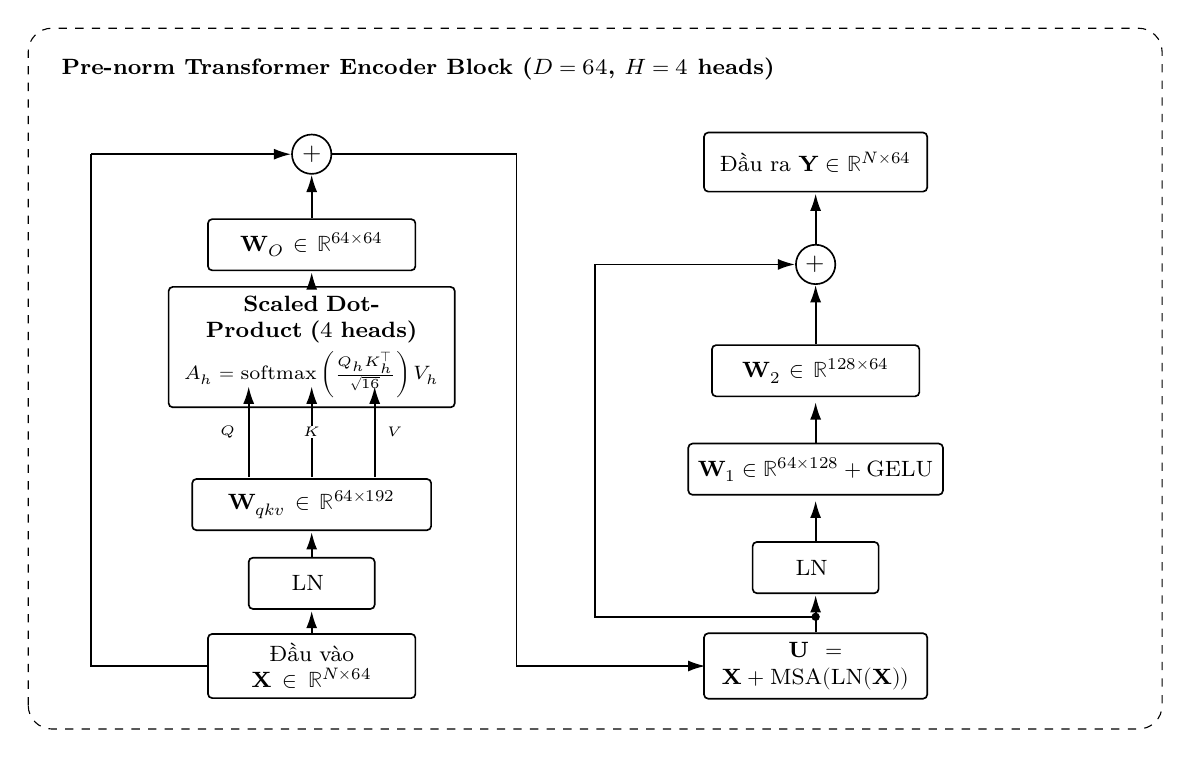
\begin{tikzpicture}[x=1cm,y=1cm]
  % Container frame
  \draw[draw=black, dashed, rounded corners=3mm, fill=white] (-1.2, -0.8) rectangle (13.2, 8.1);
  \node[font=\footnotesize\bfseries, anchor=north west] at (-0.9, 7.85) {Pre-norm Transformer Encoder Block ($D=64$, $H=4$ heads)};

  % ---------------- TOWER 1: MSA SUB-LAYER ----------------
  % Input X
  \node[arch_box_gray, text width=2.4cm, minimum height=0.75cm] (x_in) at (2.4, 0.0) {
    Đầu vào $\mathbf{X} \in \mathbb{R}^{N\times 64}$
  };

  % LN 1
  \draw[arch_arrow] (x_in.north) -- (2.4, 0.7);
  \node[arch_box, minimum width=1.6cm, minimum height=0.65cm] (ln1) at (2.4, 1.05) {
    $\mathrm{LN}$
  };

  % QKV Linear
  \draw[arch_arrow] (ln1.north) -- (2.4, 1.7);
  \node[arch_box_dark, text width=2.8cm, minimum height=0.65cm] (qkv) at (2.4, 2.05) {
    $\mathbf{W}_{qkv} \in \mathbb{R}^{64 \times 192}$
  };

  % Attention computation
  \node[arch_box_gray, text width=3.4cm, minimum height=0.95cm] (att) at (2.4, 4.05) {
    \textbf{Scaled Dot-Product ($4$ heads)}\\[2pt]
    \scriptsize $A_h = \operatorname{softmax}\left(\frac{Q_h K_h^\top}{\sqrt{16}}\right) V_h$
  };

  % Three parallel vertical arrows directly from QKV to Attention
  \draw[arch_arrow] (1.6, 2.40) -- node[left=1pt, font=\tiny] {$Q$} (1.6, 3.55);
  \draw[arch_arrow] (2.4, 2.40) -- node[fill=white, inner sep=0.5pt, font=\tiny] {$K$} (2.4, 3.55);
  \draw[arch_arrow] (3.2, 2.40) -- node[right=1pt, font=\tiny] {$V$} (3.2, 3.55);

  % Out Linear
  \draw[arch_arrow] (att.north) -- (2.4, 5.0);
  \node[arch_box, text width=2.4cm, minimum height=0.65cm] (proj) at (2.4, 5.35) {
    $\mathbf{W}_O \in \mathbb{R}^{64\times 64}$
  };

  % Addition 1
  \node[arch_op] (add1) at (2.4, 6.5) {$+$};
  \draw[arch_arrow] (proj.north) -- (add1.south);

  % Residual 1 highway
  \draw[arch_line] (x_in.west) -- (-0.4, 0.0) -- (-0.4, 6.5);
  \draw[arch_arrow] (-0.4, 6.5) -- (add1.west);

  % ---------------- BRIDGE: TOWER 1 TO TOWER 2 ----------------
  \draw[arch_line] (add1.east) -- (5.0, 6.5) -- (5.0, 0.0);
  \draw[arch_arrow] (5.0, 0.0) -- (7.4, 0.0);

  % ---------------- TOWER 2: FFN SUB-LAYER ----------------
  % Intermediate tensor U
  \node[arch_box_gray, text width=2.6cm, minimum height=0.75cm] (u_mid) at (8.8, 0.0) {
    $\mathbf{U} = \mathbf{X} + \text{MSA}(\text{LN}(\mathbf{X}))$
  };

  % LN 2
  \draw[arch_arrow] (u_mid.north) -- (8.8, 0.9);
  \node[arch_box, minimum width=1.6cm, minimum height=0.65cm] (ln2) at (8.8, 1.25) {
    $\mathrm{LN}$
  };

  % FFN 1 (widened to 3.0cm for clean single line)
  \draw[arch_arrow] (ln2.north) -- (8.8, 2.1);
  \node[arch_box, text width=3.0cm, minimum height=0.65cm] (ffn1) at (8.8, 2.5) {
    $\mathbf{W}_1 \in \mathbb{R}^{64\times 128} + \text{GELU}$
  };

  % FFN 2
  \draw[arch_arrow] (ffn1.north) -- (8.8, 3.35);
  \node[arch_box, text width=2.4cm, minimum height=0.65cm] (ffn2) at (8.8, 3.75) {
    $\mathbf{W}_2 \in \mathbb{R}^{128\times 64}$
  };

  % Addition 2
  \node[arch_op] (add2) at (8.8, 5.1) {$+$};
  \draw[arch_arrow] (ffn2.north) -- (add2.south);

  % Residual 2 highway
  \coordinate (tap_u) at (8.8, 0.625);
  \fill[black] (tap_u) circle (1.5pt);
  \draw[arch_line] (tap_u) -- (6.0, 0.625) -- (6.0, 5.1);
  \draw[arch_arrow] (6.0, 5.1) -- (add2.west);

  % Output Y
  \draw[arch_arrow] (add2.north) -- (8.8, 6.0);
  \node[arch_box_dark, text width=2.6cm, minimum height=0.75cm] (y_out) at (8.8, 6.4) {
    Đầu ra $\mathbf{Y} \in \mathbb{R}^{N\times 64}$
  };
\end{tikzpicture}}

% =============================================================
% 8. ARCHITECTURE: Recurrent Sequence
% =============================================================
\newcommand{\ArchSequence}{%
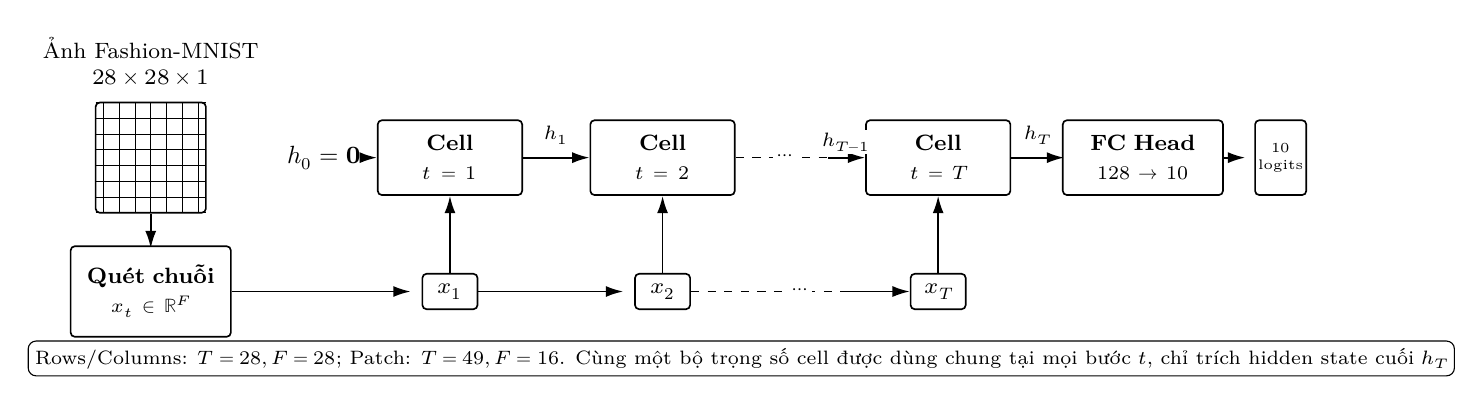
\begin{tikzpicture}[x=1cm,y=1cm]
  % Input image at top-left
  \node[arch_box, minimum width=1.4cm, minimum height=1.4cm, fill=white] (im) at (-2.2, 0.7) {};
  \draw[step=0.2cm, black, line width=0.25pt] (-2.9,0.0) grid (-1.5,1.4);
  \node[font=\footnotesize, anchor=south, align=center] at (-2.2, 1.5) {Ảnh Fashion-MNIST\\$28\times 28\times 1$};

  % Sequence generator
  \draw[arch_arrow] (im.south) -- (-2.2, -0.45);
  \node[arch_box_gray, text width=1.8cm, minimum height=1.15cm] (scan) at (-2.2, -1.0) {
    \textbf{Quét chuỗi}\\[1pt]
    \scriptsize $x_t \in \mathbb{R}^F$
  };

  % Initial state h0 (centered at 0.0 with clear separation from im at -1.5)
  \node[font=\small] (h0) at (0.0, 0.7) {$h_0 = \mathbf{0}$};

  % Step 1
  \node[arch_box, text width=1.6cm, minimum height=0.95cm] (c1) at (1.6, 0.7) {
    \textbf{Cell}\\[1pt]
    \scriptsize $t=1$
  };
  \draw[arch_arrow] (h0.east) -- (c1.west);

  \draw[arch_arrow] (scan.east) -- (1.1, -1.0);
  \node[arch_box, minimum width=0.7cm, minimum height=0.45cm] (x1) at (1.6, -1.0) {$x_1$};
  \draw[arch_arrow] (x1.north) -- (c1.south);

  % Step 2
  \node[arch_box, text width=1.6cm, minimum height=0.95cm] (c2) at (4.3, 0.7) {
    \textbf{Cell}\\[1pt]
    \scriptsize $t=2$
  };
  \draw[arch_arrow] (c1.east) -- node[above=1pt, font=\scriptsize] {$h_1$} (c2.west);

  \draw[arch_arrow] (x1.east) -- (3.8, -1.0);
  \node[arch_box, minimum width=0.7cm, minimum height=0.45cm] (x2) at (4.3, -1.0) {$x_2$};
  \draw[arch_arrow] (x2.north) -- (c2.south);

  % Step T (ellipses)
  \node[arch_box, text width=1.6cm, minimum height=0.95cm] (cT) at (7.8, 0.7) {
    \textbf{Cell}\\[1pt]
    \scriptsize $t=T$
  };

  \draw[arch_dash] (c2.east) -- (6.4, 0.7);
  \node[font=\scriptsize, fill=white, inner sep=1.5pt] at (5.85, 0.7) {$\cdots$};
  \draw[arch_arrow] (6.4, 0.7) -- node[above=1pt, font=\scriptsize, fill=white, inner sep=1pt] {$h_{T-1}$} (cT.west);

  \node[arch_box, minimum width=0.7cm, minimum height=0.45cm] (xT) at (7.8, -1.0) {$x_T$};
  \draw[arch_arrow] (xT.north) -- (cT.south);

  \draw[arch_dash] (x2.east) -- (7.3, -1.0);
  \node[font=\scriptsize, fill=white, inner sep=1.5pt] at (6.05, -1.0) {$\cdots$};
  \draw[arch_arrow] (6.6, -1.0) -- (xT.west);

  % FC Head
  \draw[arch_arrow] (cT.east) -- node[above=1pt, font=\scriptsize] {$h_T$} (9.4, 0.7);
  \node[arch_box_gray, text width=1.8cm, minimum height=0.95cm] (head) at (10.4, 0.7) {
    \textbf{FC Head}\\[1pt]
    \scriptsize $128 \to 10$
  };

  % Logits
  \draw[arch_arrow] (head.east) -- (11.7, 0.7);
  \node[arch_box_dark, minimum width=0.65cm, minimum height=0.95cm] (out) at (12.15, 0.7) {};
  \node[font=\tiny, align=center] at (12.15, 0.7) {$10$\\logits};

  % Note below
  \node[arch_badge] at (5.3, -1.85) {Rows/Columns: $T=28, F=28$; Patch: $T=49, F=16$. Cùng một bộ trọng số cell được dùng chung tại mọi bước $t$, chỉ trích hidden state cuối $h_T$};
\end{tikzpicture}}

% =============================================================
% 9. ARCHITECTURE: LSTM Cell
% =============================================================
\newcommand{\ArchLSTM}{%
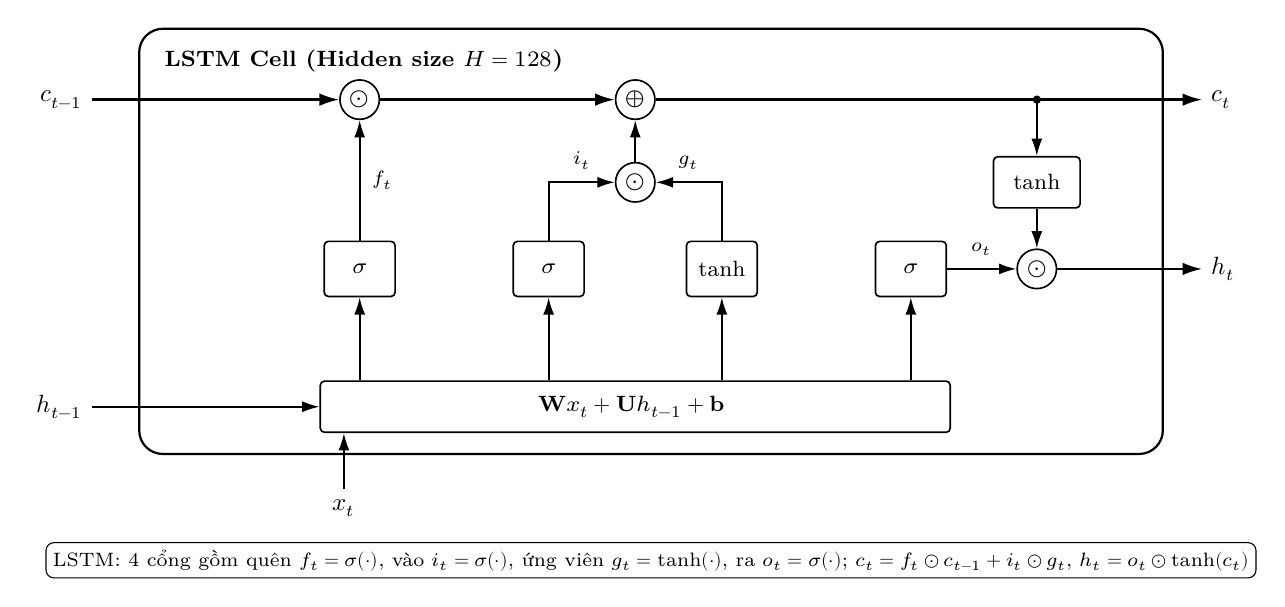
\begin{tikzpicture}[x=1cm,y=1cm]
  % Boundary of LSTM cell
  \draw[draw=black, rounded corners=3mm, line width=0.8pt, fill=white] (-0.8, -1.1) rectangle (12.2, 4.3);
  \node[font=\footnotesize\bfseries, anchor=north west] at (-0.6, 4.15) {LSTM Cell (Hidden size $H=128$)};

  % Top Cell State Highway
  \node[font=\small, anchor=east] (cp) at (-1.4, 3.4) {$c_{t-1}$};
  \node[arch_op] (mul_f) at (2.0, 3.4) {$\odot$};
  \node[arch_op] (add_c) at (5.5, 3.4) {$\oplus$};
  \node[font=\small, anchor=west] (cn) at (12.7, 3.4) {$c_t$};

  \draw[arch_arrow_thick] (cp.east) -- (mul_f.west);
  \draw[arch_arrow_thick] (mul_f.east) -- (add_c.west);
  \draw[arch_arrow_thick] (add_c.east) -- (cn.west);

  % Bottom Inputs: x_t and h_{t-1}
  \node[font=\small, anchor=east] (hp) at (-1.4, -0.5) {$h_{t-1}$};
  \node[font=\small, anchor=north] (xt) at (1.8, -1.55) {$x_t$};

  % Wide Projections Bar
  \node[arch_box_gray, minimum width=8.0cm, minimum height=0.65cm] (proj) at (5.5, -0.5) {
    $\mathbf{W}x_t + \mathbf{U}h_{t-1} + \mathbf{b}$
  };
  \draw[arch_arrow] (hp.east) -- (proj.west);
  \draw[arch_arrow] (xt.north) -- (proj.south -| xt.north);

  % 4 Parallel Gates
  \node[arch_box, minimum width=0.9cm, minimum height=0.7cm] (gf) at (2.0, 1.25) {$\sigma$};
  \node[arch_box, minimum width=0.9cm, minimum height=0.7cm] (gi) at (4.4, 1.25) {$\sigma$};
  \node[arch_box, minimum width=0.9cm, minimum height=0.7cm] (gg) at (6.6, 1.25) {$\tanh$};
  \node[arch_box, minimum width=0.9cm, minimum height=0.7cm] (go) at (9.0, 1.25) {$\sigma$};

  % Connections from projection to gates
  \draw[arch_arrow] (proj.north -| gf.south) -- (gf.south);
  \draw[arch_arrow] (proj.north -| gi.south) -- (gi.south);
  \draw[arch_arrow] (proj.north -| gg.south) -- (gg.south);
  \draw[arch_arrow] (proj.north -| go.south) -- (go.south);

  % Forget gate to Cell State
  \draw[arch_arrow] (gf.north) -- node[right=1pt, font=\scriptsize] {$f_t$} (mul_f.south);

  % Candidate multiplication (straight vertical entry to add_c)
  \node[arch_op] (mul_i) at (5.5, 2.35) {$\odot$};
  \draw[arch_arrow] (gi.north) |- node[pos=0.75, above=1pt, font=\scriptsize] {$i_t$} (mul_i.west);
  \draw[arch_arrow] (gg.north) |- node[pos=0.75, above=1pt, font=\scriptsize] {$g_t$} (mul_i.east);
  \draw[arch_arrow] (mul_i.north) -- (add_c.south);

  % Output gate & tanh on cell state
  \node[arch_box, minimum width=1.1cm, minimum height=0.65cm] (tanh_c) at (10.6, 2.35) {$\tanh$};
  \coordinate (tap_c) at (10.6, 3.4);
  \fill[black] (tap_c) circle (1.5pt);
  \draw[arch_arrow] (tap_c) -- (tanh_c.north);

  \node[arch_op] (mul_o) at (10.6, 1.25) {$\odot$};
  \draw[arch_arrow] (tanh_c.south) -- (mul_o.north);
  \draw[arch_arrow] (go.east) -- node[above=1pt, font=\scriptsize] {$o_t$} (mul_o.west);

  % Hidden state out
  \node[font=\small, anchor=west] (hn) at (12.7, 1.25) {$h_t$};
  \draw[arch_arrow_thick] (mul_o.east) -- (hn.west);

  % Explanatory badge below
  \node[arch_badge] at (5.7, -2.45) {LSTM: 4 cổng gồm quên $f_t=\sigma(\cdot)$, vào $i_t=\sigma(\cdot)$, ứng viên $g_t=\tanh(\cdot)$, ra $o_t=\sigma(\cdot)$; $c_t = f_t \odot c_{t-1} + i_t \odot g_t$, $h_t = o_t \odot \tanh(c_t)$};
\end{tikzpicture}}

% =============================================================
% 10. ARCHITECTURE: GRU Cell
% 100% PLANAR LAYOUT: ZERO INTERSECTIONS!
% =============================================================
\newcommand{\ArchGRU}{%
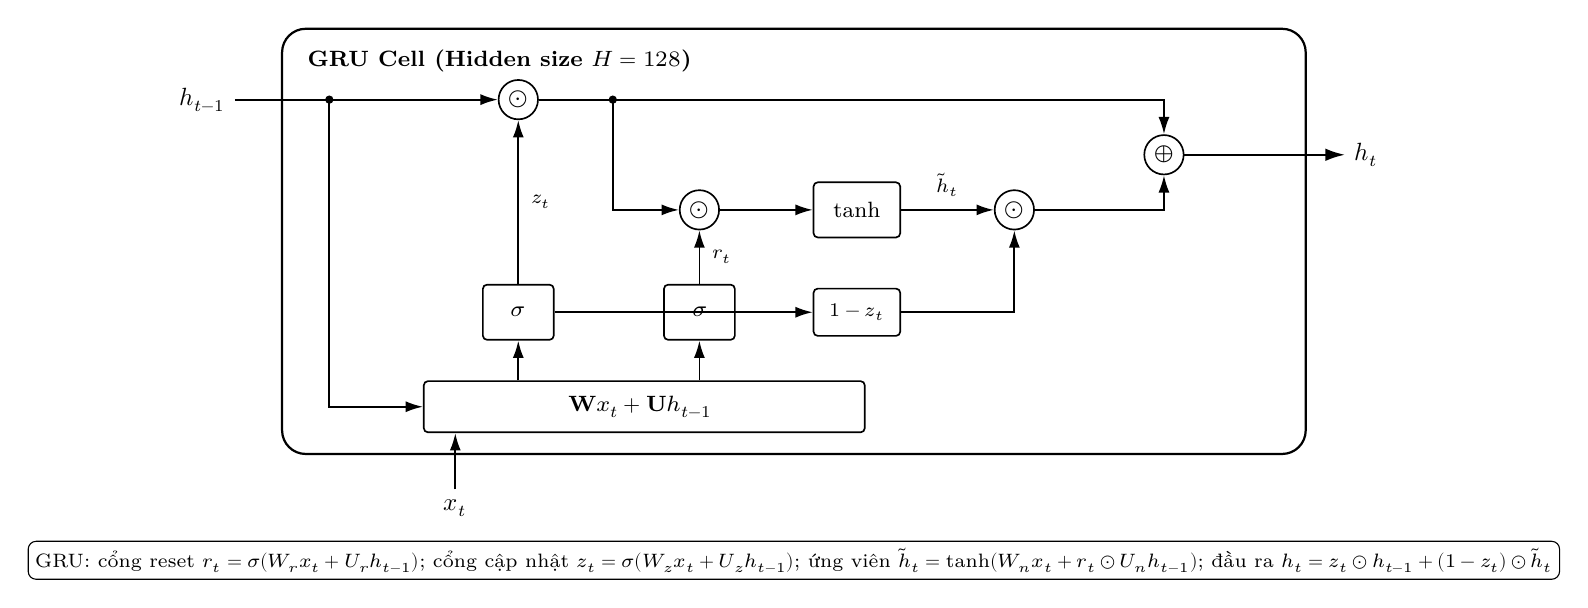
\begin{tikzpicture}[x=1cm,y=1cm]
  % Boundary of GRU cell
  \draw[draw=black, rounded corners=3mm, line width=0.8pt, fill=white] (-0.8, -1.1) rectangle (12.2, 4.3);
  \node[font=\footnotesize\bfseries, anchor=north west] at (-0.6, 4.15) {GRU Cell (Hidden size $H=128$)};

  % External Inputs
  \node[font=\small, anchor=east] (hp) at (-1.4, 3.4) {$h_{t-1}$};
  \node[font=\small, anchor=north] (xt) at (1.4, -1.55) {$x_t$};

  % Wide Linear Projections Bar
  \node[arch_box_gray, minimum width=5.6cm, minimum height=0.65cm] (proj) at (3.8, -0.5) {
    $\mathbf{W}x_t + \mathbf{U}h_{t-1}$
  };
  \draw[arch_arrow] (xt.north) -- (proj.south -| xt.north);

  % h_{t-1} branch down to proj.west at x = -0.2
  \coordinate (tap_p) at (-0.2, 3.4);
  \fill[black] (tap_p) circle (1.5pt);
  \draw[arch_arrow] (tap_p) |- (proj.west);

  % 1. Update Gate z_t on Left (x = 2.2)
  \node[arch_box, minimum width=0.9cm, minimum height=0.7cm] (gz) at (2.2, 0.7) {$\sigma$};
  \draw[arch_arrow] (proj.north -| gz.south) -- (gz.south);

  % mul_keep: z_t * h_{t-1} directly on highway at (2.2, 3.4)
  \node[arch_op] (mul_keep) at (2.2, 3.4) {$\odot$};
  \draw[arch_arrow] (hp.east) -- (mul_keep.west);
  \draw[arch_arrow] (gz.north) -- node[right=1pt, font=\scriptsize] {$z_t$} (mul_keep.south);

  % 2. Reset Gate r_t in Middle (x = 4.5)
  \node[arch_box, minimum width=0.9cm, minimum height=0.7cm] (gr) at (4.5, 0.7) {$\sigma$};
  \draw[arch_arrow] (proj.north -| gr.south) -- (gr.south);

  % mul_r at (4.5, 2.0)
  \node[arch_op] (mul_r) at (4.5, 2.0) {$\odot$};
  \draw[arch_arrow] (gr.north) -- node[right=1pt, font=\scriptsize] {$r_t$} (mul_r.south);

  % h_{t-1} tap to mul_r at x = 3.4
  \coordinate (tap_r) at (3.4, 3.4);
  \fill[black] (tap_r) circle (1.5pt);
  \draw[arch_arrow] (tap_r) |- (mul_r.west);

  % 3. Candidate Cell gn (\tanh) at (6.5, 2.0)
  \node[arch_box, minimum width=1.1cm, minimum height=0.7cm] (gn) at (6.5, 2.0) {$\tanh$};
  \draw[arch_arrow] (mul_r.east) -- (gn.west);

  % Blend box: (1 - z_t) at (6.5, 0.7)
  \node[arch_box, minimum width=1.1cm, minimum height=0.6cm] (inv_z) at (6.5, 0.7) {\scriptsize $1 - z_t$};
  \draw[arch_arrow] (gz.east) -- (inv_z.west);

  % 4. Candidate Multiplier at (8.5, 2.0): (1 - z_t) * \tilde{h}_t
  \node[arch_op] (mul_cand) at (8.5, 2.0) {$\odot$};
  \draw[arch_arrow] (gn.east) -- node[above=1pt, font=\scriptsize] {$\tilde{h}_t$} (mul_cand.west);
  \draw[arch_arrow] (inv_z.east) -| (mul_cand.south);

  % 5. Output Addition at (10.4, 2.7)
  \node[arch_op] (add_h) at (10.4, 2.7) {$\oplus$};
  \draw[arch_arrow] (mul_keep.east) -| (add_h.north);
  \draw[arch_arrow] (mul_cand.east) -| (add_h.south);

  % Output h_t
  \node[font=\small, anchor=west] (hn) at (12.7, 2.7) {$h_t$};
  \draw[arch_arrow_thick] (add_h.east) -- (hn.west);

  % Explanatory badge below
  \node[arch_badge] at (5.7, -2.45) {GRU: cổng reset $r_t = \sigma(W_r x_t + U_r h_{t-1})$; cổng cập nhật $z_t = \sigma(W_z x_t + U_z h_{t-1})$; ứng viên $\tilde{h}_t = \tanh(W_n x_t + r_t \odot U_n h_{t-1})$; đầu ra $h_t = z_t \odot h_{t-1} + (1 - z_t) \odot \tilde{h}_t$};
\end{tikzpicture}}

% =============================================================
% 11. ARCHITECTURE: ResNet-50
% =============================================================
\newcommand{\ArchResNet}{%
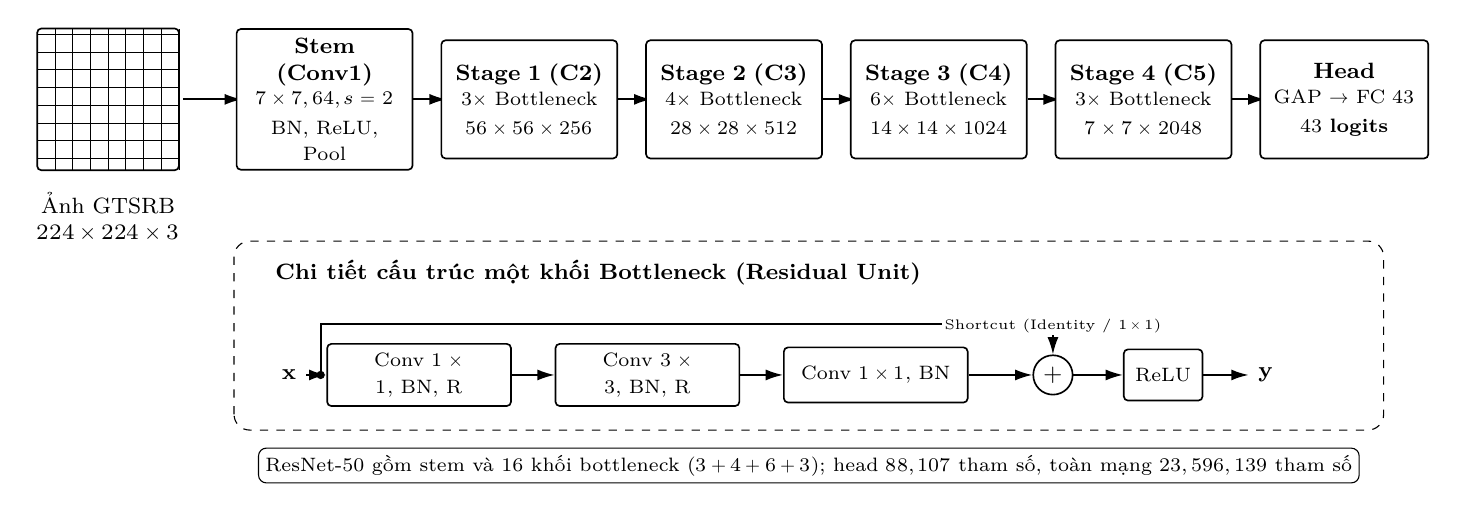
\begin{tikzpicture}[x=1cm,y=1cm]
  \def\ty{3.0}

  % Input image
  \node[arch_box, minimum width=1.8cm, minimum height=1.8cm, fill=white] (in) at (0, \ty) {};
  \draw[step=0.225cm, black, line width=0.25pt] (-0.9,2.1) grid (0.9,3.9);
  \node[font=\footnotesize, anchor=north, align=center] at (0, 1.95) {Ảnh GTSRB\\$224\times 224\times 3$};

  % Stem
  \draw[arch_arrow] (0.95, \ty) -- (1.7, \ty);
  \node[arch_box, text width=2.0cm, minimum height=1.5cm] (stem) at (2.75, \ty) {
    \textbf{Stem (Conv1)}\\[1pt]
    \scriptsize $7\times 7, 64, s=2$\\[1pt]
    BN, ReLU, Pool
  };

  % Stage 1 (C2)
  \draw[arch_arrow] (stem.east) -- (4.3, \ty);
  \node[arch_box_gray, text width=2.0cm, minimum height=1.5cm] (c2) at (5.35, \ty) {
    \textbf{Stage 1 (C2)}\\[1pt]
    \scriptsize $3\times$ Bottleneck\\[1pt]
    \textbf{$56\times 56\times 256$}
  };

  % Stage 2 (C3)
  \draw[arch_arrow] (c2.east) -- (6.9, \ty);
  \node[arch_box_gray, text width=2.0cm, minimum height=1.5cm] (c3) at (7.95, \ty) {
    \textbf{Stage 2 (C3)}\\[1pt]
    \scriptsize $4\times$ Bottleneck\\[1pt]
    \textbf{$28\times 28\times 512$}
  };

  % Stage 3 (C4)
  \draw[arch_arrow] (c3.east) -- (9.5, \ty);
  \node[arch_box_gray, text width=2.0cm, minimum height=1.5cm] (c4) at (10.55, \ty) {
    \textbf{Stage 3 (C4)}\\[1pt]
    \scriptsize $6\times$ Bottleneck\\[1pt]
    \textbf{$14\times 14\times 1024$}
  };

  % Stage 4 (C5)
  \draw[arch_arrow] (c4.east) -- (12.1, \ty);
  \node[arch_box_gray, text width=2.0cm, minimum height=1.5cm] (c5) at (13.15, \ty) {
    \textbf{Stage 4 (C5)}\\[1pt]
    \scriptsize $3\times$ Bottleneck\\[1pt]
    \textbf{$7\times 7\times 2048$}
  };

  % Classification Head
  \draw[arch_arrow] (c5.east) -- (14.7, \ty);
  \node[arch_box_dark, text width=1.9cm, minimum height=1.5cm] (head) at (15.7, \ty) {
    \textbf{Head}\\[1pt]
    \scriptsize GAP $\to$ FC $43$\\[1pt]
    \textbf{$43$ logits}
  };

  % Inset Detail: Bottleneck Block
  \draw[draw=black, dashed, rounded corners=2mm, fill=white] (1.6, -1.2) rectangle (16.2, 1.2);
  \node[font=\footnotesize\bfseries, anchor=west] at (2.0, 0.8) {Chi tiết cấu trúc một khối Bottleneck (Residual Unit)};

  \def\by{-0.5}
  \node[font=\footnotesize] (bx_in) at (2.3, \by) {$\mathbf{x}$};
  \node[arch_box, text width=2.1cm, minimum height=0.7cm] (b_c1) at (3.95, \by) {\scriptsize Conv $1\times 1$, BN, R};
  \node[arch_box, text width=2.1cm, minimum height=0.7cm] (b_c2) at (6.85, \by) {\scriptsize Conv $3\times 3$, BN, R};
  \node[arch_box, text width=2.1cm, minimum height=0.7cm] (b_c3) at (9.75, \by) {\scriptsize Conv $1\times 1$, BN};
  \node[arch_op] (b_add) at (12.0, \by) {$+$};
  \node[arch_box, minimum width=1.0cm, minimum height=0.65cm] (b_relu) at (13.4, \by) {\scriptsize ReLU};
  \node[font=\footnotesize] (bx_out) at (14.7, \by) {$\mathbf{y}$};

  \draw[arch_arrow] (bx_in) -- (b_c1);
  \draw[arch_arrow] (b_c1) -- (b_c2);
  \draw[arch_arrow] (b_c2) -- (b_c3);
  \draw[arch_arrow] (b_c3) -- (b_add);
  \draw[arch_arrow] (b_add) -- (b_relu);
  \draw[arch_arrow] (b_relu) -- (bx_out);

  % Residual shortcut
  \coordinate (b_tap) at (2.7, \by);
  \fill[black] (b_tap) circle (1.5pt);
  \draw[arch_line] (b_tap) -- (2.7, 0.15) -- (12.0, 0.15);
  \draw[arch_arrow] (12.0, 0.15) -- node[above=1pt, font=\tiny, fill=white, inner sep=1pt] {Shortcut (Identity / $1\times 1$)} (b_add.north);

  % Overall capacity badge
  \node[arch_badge] at (8.9, -1.65) {ResNet-50 gồm stem và 16 khối bottleneck ($3+4+6+3$); head $88,107$ tham số, toàn mạng $23,596,139$ tham số};
\end{tikzpicture}}

% =============================================================
% 12. ARCHITECTURE: DeiT-Small/16
% =============================================================
\newcommand{\ArchDeiT}{%
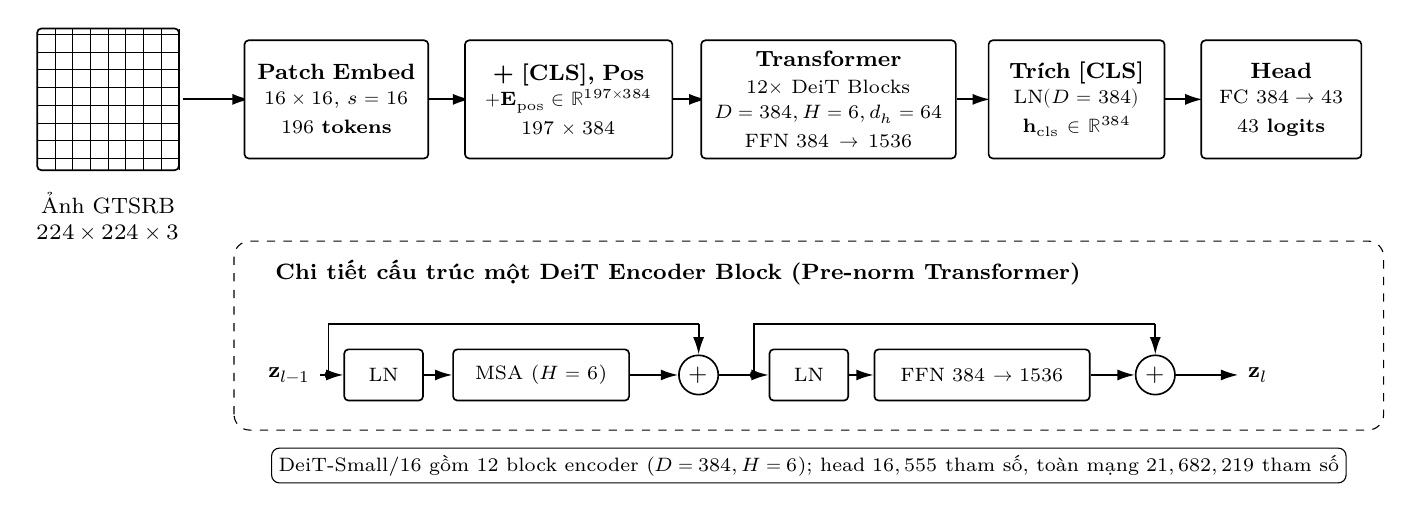
\begin{tikzpicture}[x=1cm,y=1cm]
  \def\ty{3.0}

  % Input image
  \node[arch_box, minimum width=1.8cm, minimum height=1.8cm, fill=white] (in) at (0, \ty) {};
  \draw[step=0.225cm, black, line width=0.25pt] (-0.9,2.1) grid (0.9,3.9);
  \node[font=\footnotesize, anchor=north, align=center] at (0, 1.95) {Ảnh GTSRB\\$224\times 224\times 3$};

  % Patch Embedding
  \draw[arch_arrow] (0.95, \ty) -- (1.8, \ty);
  \node[arch_box, text width=2.1cm, minimum height=1.5cm] (pe) at (2.9, \ty) {
    \textbf{Patch Embed}\\[1pt]
    \scriptsize $16\times 16$, $s=16$\\[1pt]
    \textbf{$196$ tokens}
  };

  % CLS + Pos Embedding
  \draw[arch_arrow] (pe.east) -- (4.6, \ty);
  \node[arch_box_gray, text width=2.4cm, minimum height=1.5cm] (cls_pos) at (5.85, \ty) {
    \textbf{+ [CLS], Pos}\\[1pt]
    \scriptsize $+\mathbf{E}_{\mathrm{pos}} \in \mathbb{R}^{197\times 384}$\\[1pt]
    \textbf{$197\times 384$}
  };

  % 12 Transformer Encoder Blocks
  \draw[arch_arrow] (cls_pos.east) -- (7.6, \ty);
  \node[arch_box_dark, text width=3.0cm, minimum height=1.5cm] (enc) at (9.15, \ty) {
    \textbf{Transformer}\\[2pt]
    \scriptsize $12\times$ DeiT Blocks\\[1pt]
    $D=384, H=6, d_h=64$\\[1pt]
    $\text{FFN } 384\to 1536$
  };

  % Extract CLS & LayerNorm
  \draw[arch_arrow] (enc.east) -- (11.2, \ty);
  \node[arch_box, text width=2.0cm, minimum height=1.5cm] (ext) at (12.3, \ty) {
    \textbf{Trích [CLS]}\\[1pt]
    \scriptsize $\mathrm{LN} (D=384)$\\[1pt]
    $\mathbf{h}_{\mathrm{cls}} \in \mathbb{R}^{384}$
  };

  % Classification Head
  \draw[arch_arrow] (ext.east) -- (13.9, \ty);
  \node[arch_box_gray, text width=1.8cm, minimum height=1.5cm] (head) at (14.9, \ty) {
    \textbf{Head}\\[1pt]
    \scriptsize FC $384 \to 43$\\[1pt]
    \textbf{$43$ logits}
  };

  % Inset Detail: DeiT Block
  \draw[draw=black, dashed, rounded corners=2mm, fill=white] (1.6, -1.2) rectangle (16.2, 1.2);
  \node[font=\footnotesize\bfseries, anchor=west] at (2.0, 0.8) {Chi tiết cấu trúc một DeiT Encoder Block (Pre-norm Transformer)};

  \def\by{-0.5}
  \node[font=\footnotesize] (dx_in) at (2.3, \by) {$\mathbf{z}_{l-1}$};
  \node[arch_box, minimum width=1.0cm, minimum height=0.65cm] (d_ln1) at (3.5, \by) {\scriptsize LN};
  \node[arch_box, text width=2.0cm, minimum height=0.65cm] (d_msa) at (5.5, \by) {\scriptsize MSA ($H=6$)};
  \node[arch_op] (d_add1) at (7.5, \by) {$+$};
  \node[arch_box, minimum width=1.0cm, minimum height=0.65cm] (d_ln2) at (8.9, \by) {\scriptsize LN};
  \node[arch_box, text width=2.5cm, minimum height=0.65cm] (d_ffn) at (11.1, \by) {\scriptsize FFN $384\to 1536$};
  \node[arch_op] (d_add2) at (13.3, \by) {$+$};
  \node[font=\footnotesize] (dx_out) at (14.6, \by) {$\mathbf{z}_l$};

  \draw[arch_arrow] (dx_in) -- (d_ln1);
  \draw[arch_arrow] (d_ln1) -- (d_msa);
  \draw[arch_arrow] (d_msa) -- (d_add1);
  \draw[arch_arrow] (d_add1) -- (d_ln2);
  \draw[arch_arrow] (d_ln2) -- (d_ffn);
  \draw[arch_arrow] (d_ffn) -- (d_add2);
  \draw[arch_arrow] (d_add2) -- (dx_out);

  % Residual connections in block
  \coordinate (d_tap1) at (2.8, \by);
  \fill[black] (d_tap1) circle (1.5pt);
  \draw[arch_line] (d_tap1) -- (2.8, 0.15) -- (7.5, 0.15);
  \draw[arch_arrow] (7.5, 0.15) -- (d_add1.north);

  \coordinate (d_tap2) at (8.2, \by);
  \fill[black] (d_tap2) circle (1.5pt);
  \draw[arch_line] (d_tap2) -- (8.2, 0.15) -- (13.3, 0.15);
  \draw[arch_arrow] (13.3, 0.15) -- (d_add2.north);

  % Capacity note
  \node[arch_badge] at (8.9, -1.65) {DeiT-Small/16 gồm 12 block encoder ($D=384, H=6$); head $16,555$ tham số, toàn mạng $21,682,219$ tham số};
\end{tikzpicture}}

% =============================================================
% 13. ARCHITECTURE: FPN
% Parameter #1 = 1: RetinaNet (P3--P7)
% Parameter #1 = 2: Faster R-CNN (P2--P6)
% =============================================================
\newcommand{\ArchFPN}[1]{%
\begin{tikzpicture}[x=1cm,y=1cm]
  % Column Headers
  \node[arch_title] at (0.8, 10.3) {ResNet-50\\(Bottom-up)};
  \node[arch_title] at (5.0, 10.3) {Top-down pathway\\$T_l = \text{Conv}_{1\times 1}(C_l) + \uparrow T_{l+1}$};
  \node[arch_title] at (9.2, 10.3) {Feature Pyramid\\(Smoothing $3\times 3$)};

  % Level 5 (Exact horizontal axis at y = 8.55)
  \TensorMap{c5}{0}{8.2}{0.7}{0.7}{0.9}{0.8}{}
  \node[font=\footnotesize, anchor=east] at (-0.2, 8.55) {$C_5: 16^2\times 2048$};
  \node[arch_box_gray, minimum width=1.1cm, minimum height=0.65cm] (t5) at (5.0, 8.55) {$T_5$};
  \draw[arch_arrow] (0.7, 8.55) -- node[above=1pt, font=\scriptsize, fill=white, inner sep=1pt] {Conv $1\times 1$} (t5.west);
  \TensorMap{p5}{8.5}{8.2}{0.7}{0.7}{0.45}{0.7}{}
  \node[font=\footnotesize, anchor=west] at (9.8, 8.55) {$P_5: 16^2\times 256$};
  \draw[arch_arrow] (t5.east) -- node[above=1pt, font=\scriptsize, fill=white, inner sep=1pt] {Conv $3\times 3$} (8.5, 8.55);

  % Level 4 (Exact horizontal axis at y = 6.25)
  \TensorMap{c4}{0}{5.8}{0.9}{0.9}{0.75}{0.7}{}
  \node[font=\footnotesize, anchor=east] at (-0.2, 6.25) {$C_4: 32^2\times 1024$};
  \node[arch_op] (add4) at (5.0, 6.25) {$+$};
  \draw[arch_arrow] (0.9, 6.25) -- node[above=1pt, font=\scriptsize, fill=white, inner sep=1pt] {Conv $1\times 1$} (add4.west);
  \TensorMap{p4}{8.5}{5.8}{0.9}{0.9}{0.45}{0.7}{}
  \node[font=\footnotesize, anchor=west] at (10.0, 6.25) {$P_4: 32^2\times 256$};
  \draw[arch_arrow] (add4.east) -- node[above=1pt, font=\scriptsize, fill=white, inner sep=1pt] {Conv $3\times 3$} (8.5, 6.25);
  \draw[arch_arrow] (t5.south) -- node[right=1pt, font=\scriptsize, fill=white, inner sep=1pt] {Nearest $\uparrow 2\times$} (add4.north);

  % Level 3 (Exact horizontal axis at y = 3.975)
  \TensorMap{c3}{0}{3.4}{1.15}{1.15}{0.6}{0.65}{}
  \node[font=\footnotesize, anchor=east] at (-0.2, 3.975) {$C_3: 64^2\times 512$};
  \node[arch_op] (add3) at (5.0, 3.975) {$+$};
  \draw[arch_arrow] (1.15, 3.975) -- node[above=1pt, font=\scriptsize, fill=white, inner sep=1pt] {Conv $1\times 1$} (add3.west);
  \TensorMap{p3}{8.5}{3.4}{1.15}{1.15}{0.45}{0.7}{}
  \node[font=\footnotesize, anchor=west] at (10.25, 3.975) {$P_3: 64^2\times 256$};
  \draw[arch_arrow] (add3.east) -- node[above=1pt, font=\scriptsize, fill=white, inner sep=1pt] {Conv $3\times 3$} (8.5, 3.975);
  \draw[arch_arrow] (add4.south) -- node[right=1pt, font=\scriptsize, fill=white, inner sep=1pt] {Nearest $\uparrow 2\times$} (add3.north);

  % Bottom-up backbone connection arrows between cubes
  \draw[arch_arrow] (0.575, 4.85) -- node[right=2pt, font=\scriptsize] {stride 2} (0.575, 5.8);
  \draw[arch_arrow] (0.45, 7.05) -- node[right=2pt, font=\scriptsize] {stride 2} (0.45, 8.2);

  % Conditional Level 2 and High-level extensions
  \ifnum#1=1
    % RetinaNet: P3--P7 (No C2/P2; P6 and P7 added)
    \TensorMap{p6}{8.5}{1.2}{0.55}{0.55}{0.45}{0.7}{}
    \node[font=\footnotesize, anchor=west] at (9.6, 1.45) {$P_6: 8^2\times 256$};
    \draw[arch_line] (0.35, 9.35) -- (0.35, 9.6) -- (-3.2, 9.6) -- (-3.2, 1.45);
    \draw[arch_arrow] (-3.2, 1.45) -- node[above=1pt, font=\scriptsize, fill=white, inner sep=1pt] {Conv $3\times 3$, stride 2 (từ $C_5$)} (8.5, 1.45);

    % P7 from P6 via ReLU + Conv 3x3 s=2
    \TensorMap{p7}{8.575}{-1.0}{0.4}{0.4}{0.45}{0.7}{}
    \node[font=\footnotesize, anchor=west] at (9.5, -0.8) {$P_7: 4^2\times 256$};
    \draw[arch_arrow] (8.775, 1.2) -- node[right=1pt, font=\scriptsize, fill=white, inner sep=1pt] {ReLU $\to$ Conv $3\times 3$, stride 2} (8.775, -0.46);

    \node[arch_badge] at (4.5, -2.2) {FPN trong RetinaNet sử dụng 5 mức $P_3$--$P_7$ để bao phủ các kích thước vật thể từ nhỏ đến rất lớn};

  \else
    % Faster R-CNN: P2--P6 (Includes C2 and P2; P6 from P5 via MaxPool)
    % Level 2 (Exact horizontal axis at y = 1.725)
    \TensorMap{c2}{0}{1.0}{1.45}{1.45}{0.45}{0.6}{}
    \node[font=\footnotesize, anchor=east] at (-0.2, 1.725) {$C_2: 128^2\times 256$};
    \node[arch_op] (add2) at (5.0, 1.725) {$+$};
    \draw[arch_arrow] (1.45, 1.725) -- node[above=1pt, font=\scriptsize, fill=white, inner sep=1pt] {Conv $1\times 1$} (add2.west);
    \TensorMap{p2}{8.5}{1.0}{1.45}{1.45}{0.45}{0.7}{}
    \node[font=\footnotesize, anchor=west] at (10.5, 1.725) {$P_2: 128^2\times 256$};
    \draw[arch_arrow] (add2.east) -- node[above=1pt, font=\scriptsize, fill=white, inner sep=1pt] {Conv $3\times 3$} (8.5, 1.725);
    \draw[arch_arrow] (add3.south) -- node[right=1pt, font=\scriptsize, fill=white, inner sep=1pt] {Nearest $\uparrow 2\times$} (add2.north);
    \draw[arch_arrow] (0.725, 2.65) -- node[right=2pt, font=\scriptsize] {stride 2} (0.725, 3.4);

    % P6 from P5 via MaxPool
    \TensorMap{p6}{8.5}{-1.2}{0.55}{0.55}{0.45}{0.7}{}
    \node[font=\footnotesize, anchor=north] at (8.775, -1.35) {$P_6: 8^2\times 256$};
    \draw[arch_line] (8.985, 9.075) -- (8.985, 9.4) -- (13.8, 9.4) -- (13.8, -0.925);
    \draw[arch_arrow] (13.8, -0.925) -- node[above=1pt, font=\scriptsize, fill=white, inner sep=1pt] {MaxPool $1\times 1$, stride 2 (từ $P_5$)} (9.05, -0.925);

    \node[arch_badge] at (4.5, -2.6) {FPN trong Faster R-CNN bổ sung $P_2$ độ phân giải cao cho vật thể nhỏ; $P_6$ được dùng riêng cho RPN};
  \fi
\end{tikzpicture}}

% =============================================================
% 14. ARCHITECTURE: RetinaNet Head
% =============================================================
\newcommand{\ArchRetinaHead}{%
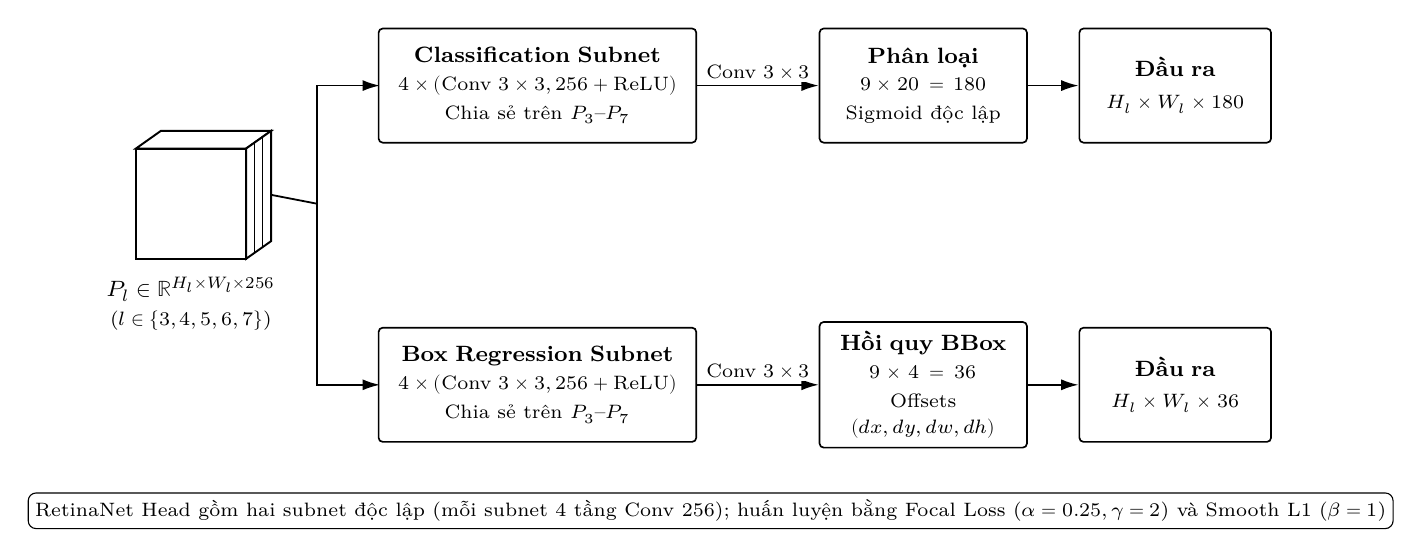
\begin{tikzpicture}[x=1cm,y=1cm]
  % Input FPN Feature Map Pl
  \TensorMap{p}{-0.5}{0.8}{1.4}{1.4}{0.45}{0.7}{$P_l \in \mathbb{R}^{H_l\times W_l\times 256}$\\[1pt]\scriptsize($l \in \{3,4,5,6,7\}$)}

  % Fork to Classification Subnet (Top) and Regression Subnet (Bottom)
  \draw[arch_line] (p-east) -- (1.8, 1.5);
  \draw[arch_arrow] (1.8, 1.5) |- (2.6, 3.0);
  \draw[arch_arrow] (1.8, 1.5) |- (2.6, -0.8);

  % Top Branch: Classification Subnet
  \node[arch_box_gray, text width=3.8cm, minimum height=1.45cm] (c_sub) at (4.6, 3.0) {
    \textbf{Classification Subnet}\\[2pt]
    \scriptsize $4\times (\text{Conv } 3\times 3, 256 + \text{ReLU})$\\[1pt]
    Chia sẻ trên $P_3$--$P_7$
  };

  \node[arch_box_dark, text width=2.4cm, minimum height=1.45cm] (c_out) at (9.5, 3.0) {
    \textbf{Phân loại}\\[2pt]
    \scriptsize $9 \times 20 = 180$\\[1pt]
    Sigmoid độc lập
  };
  \draw[arch_arrow] (c_sub.east) -- node[above=1pt, font=\scriptsize, fill=white, inner sep=1pt] {Conv $3\times 3$} (c_out.west);

  \node[arch_box, text width=2.2cm, minimum height=1.45cm, fill=white] (c_t) at (12.7, 3.0) {
    \textbf{Đầu ra}\\[2pt]
    \scriptsize $H_l\times W_l\times 180$
  };
  \draw[arch_arrow] (c_out.east) -- (c_t.west);

  % Bottom Branch: Box Regression Subnet
  \node[arch_box_gray, text width=3.8cm, minimum height=1.45cm] (r_sub) at (4.6, -0.8) {
    \textbf{Box Regression Subnet}\\[2pt]
    \scriptsize $4\times (\text{Conv } 3\times 3, 256 + \text{ReLU})$\\[1pt]
    Chia sẻ trên $P_3$--$P_7$
  };

  \node[arch_box_dark, text width=2.4cm, minimum height=1.45cm] (r_out) at (9.5, -0.8) {
    \textbf{Hồi quy BBox}\\[2pt]
    \scriptsize $9 \times 4 = 36$\\[1pt]
    Offsets $(dx, dy, dw, dh)$
  };
  \draw[arch_arrow] (r_sub.east) -- node[above=1pt, font=\scriptsize, fill=white, inner sep=1pt] {Conv $3\times 3$} (r_out.west);

  \node[arch_box, text width=2.2cm, minimum height=1.45cm, fill=white] (r_t) at (12.7, -0.8) {
    \textbf{Đầu ra}\\[2pt]
    \scriptsize $H_l\times W_l\times 36$
  };
  \draw[arch_arrow] (r_out.east) -- (r_t.west);

  % Note below
  \node[arch_badge] at (6.8, -2.4) {RetinaNet Head gồm hai subnet độc lập (mỗi subnet 4 tầng Conv 256); huấn luyện bằng Focal Loss ($\alpha=0.25, \gamma=2$) và Smooth L1 ($\beta=1$)};
\end{tikzpicture}}

% =============================================================
% 15. ARCHITECTURE: Faster R-CNN Head
% =============================================================
\newcommand{\ArchFasterHead}{%
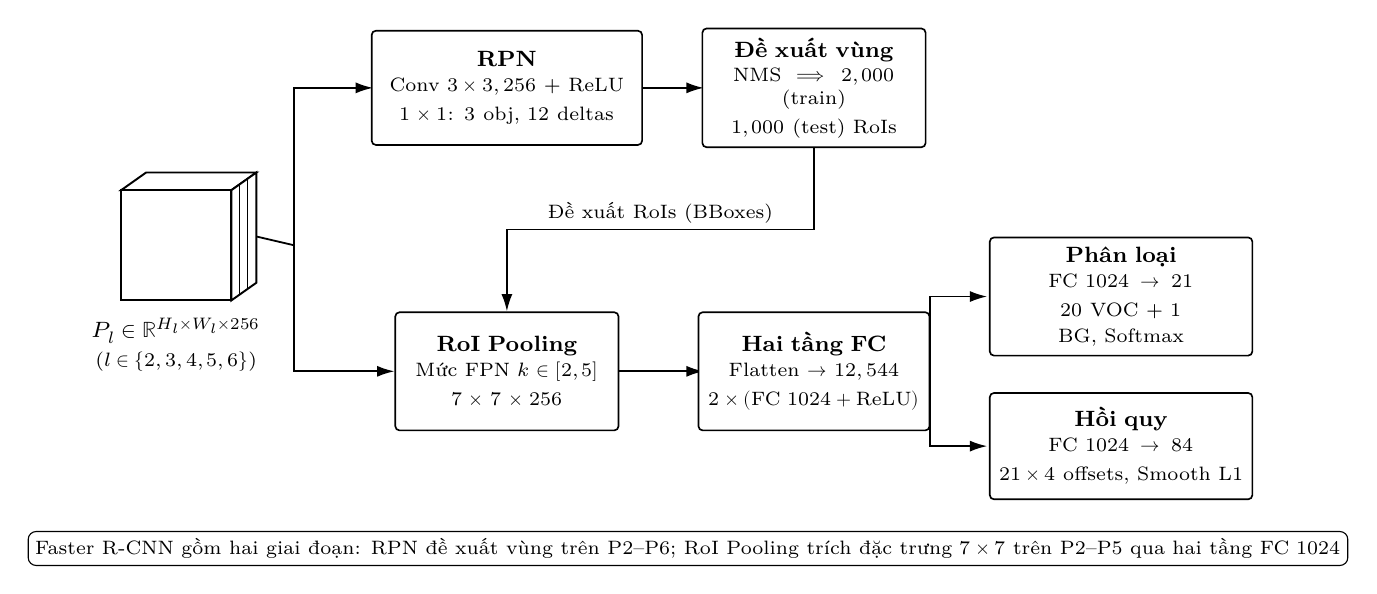
\begin{tikzpicture}[x=1cm,y=1cm]
  % Input FPN Feature Map
  \TensorMap{p}{-0.4}{1.5}{1.4}{1.4}{0.45}{0.7}{$P_l \in \mathbb{R}^{H_l\times W_l\times 256}$\\[1pt]\scriptsize($l \in \{2,3,4,5,6\}$)}

  % Branch 1: RPN (Top row at y = 4.2)
  \draw[arch_line] (p-east) -- (1.8, 2.2);
  \draw[arch_arrow] (1.8, 2.2) |- (2.8, 4.2);

  \node[arch_box_gray, text width=3.2cm, minimum height=1.45cm] (rpn) at (4.5, 4.2) {
    \textbf{RPN}\\[1pt]
    \scriptsize Conv $3\times 3, 256$ + ReLU\\[1pt]
    $1\times 1$: $3$ obj, $12$ deltas
  };

  \draw[arch_arrow] (rpn.east) -- (7.0, 4.2);
  \node[arch_box, text width=2.6cm, minimum height=1.45cm] (props) at (8.4, 4.2) {
    \textbf{Đề xuất vùng}\\[1pt]
    \scriptsize NMS $\implies 2,000$ (train)\\[1pt]
    $1,000$ (test) RoIs
  };

  % Branch 2: RoI Pooling & Head (Bottom row at y = 0.6)
  \node[arch_box_dark, text width=2.6cm, minimum height=1.5cm] (roipool) at (4.5, 0.6) {
    \textbf{RoI Pooling}\\[1pt]
    \scriptsize Mức FPN $k \in [2,5]$\\[1pt]
    \textbf{$7\times 7\times 256$}
  };
  \draw[arch_arrow] (1.8, 2.2) |- (roipool.west);

  % Proposal line from RPN: drops from props.south at y=3.475 to corridor at y=2.4, then left into roipool.north
  \draw[arch_line] (props.south) -- (8.4, 2.4);
  \draw[arch_arrow] (8.4, 2.4) -- node[above=1pt, font=\scriptsize, fill=white, inner sep=1pt] {Đề xuất RoIs (BBoxes)} (4.5, 2.4) -- (roipool.north);

  % Flatten & Two FC layers
  \draw[arch_arrow] (roipool.east) -- (7.0, 0.6);
  \node[arch_box_gray, text width=2.7cm, minimum height=1.5cm] (fcs) at (8.4, 0.6) {
    \textbf{Hai tầng FC}\\[1pt]
    \scriptsize Flatten $\to 12,544$\\[1pt]
    $2\times (\text{FC } 1024 + \text{ReLU})$
  };

  % Final dual outputs (Classification & Bbox) with 0.5cm vertical separation
  \draw[arch_arrow] (fcs.east) |- (10.6, 1.55);
  \draw[arch_arrow] (fcs.east) |- (10.6, -0.35);

  \node[arch_box, text width=3.1cm, minimum height=1.35cm] (out_cls) at (12.3, 1.55) {
    \textbf{Phân loại}\\[1pt]
    \scriptsize FC $1024 \to 21$\\[1pt]
    $20$ VOC + $1$ BG, Softmax
  };

  \node[arch_box, text width=3.1cm, minimum height=1.35cm] (out_reg) at (12.3, -0.35) {
    \textbf{Hồi quy}\\[1pt]
    \scriptsize FC $1024 \to 84$\\[1pt]
    $21 \times 4$ offsets, Smooth L1
  };

  % Note below
  \node[arch_badge] at (6.8, -1.65) {Faster R-CNN gồm hai giai đoạn: RPN đề xuất vùng trên P2--P6; RoI Pooling trích đặc trưng $7\times 7$ trên P2--P5 qua hai tầng FC $1024$};
\end{tikzpicture}}


\newcommand{\PortraitFigure}[2]{\begin{figure}[H]\centering
\makebox[\linewidth][c]{\includegraphics[width=1.13\linewidth,height=.82\textheight,keepaspectratio]{#1}}
\caption{#2}\label{fig:#1}\end{figure}}

\newcommand{\PortraitFigureIntro}[3]{#1\PortraitFigure{#2}{#3}}

% Independent assets are composed in LaTeX; the raster files are not cropped.
\setcounter{topnumber}{3}
\setcounter{bottomnumber}{2}
\setcounter{totalnumber}{4}
\renewcommand{\topfraction}{.95}
\renewcommand{\bottomfraction}{.85}
\renewcommand{\textfraction}{.05}
\renewcommand{\floatpagefraction}{.70}
\captionsetup[subfigure]{font=small,labelfont=bf,justification=centering,skip=2pt}
\newcommand{\PairFigure}[7][.39]{\begin{figure}[H]\centering
  \begin{subfigure}{\linewidth}\centering
    \includegraphics[width=.97\linewidth,height=#1\textheight,keepaspectratio]{#2}
    \caption{#3}\label{fig:#7:a}
  \end{subfigure}\par\smallskip
  \begin{subfigure}{\linewidth}\centering
    \includegraphics[width=.97\linewidth,height=#1\textheight,keepaspectratio]{#4}
    \caption{#5}\label{fig:#7:b}
  \end{subfigure}
  \caption{#6}\label{fig:#7}
\end{figure}}
\newcommand{\ArchitecturePair}[6]{\begin{figure}[htbp]\centering
  \begin{subfigure}{\linewidth}\centering
    \resizebox{.97\linewidth}{!}{#1}\caption{#2}\label{fig:#6:a}
  \end{subfigure}\par\medskip
  \begin{subfigure}{\linewidth}\centering
    \resizebox{.97\linewidth}{!}{#3}\caption{#4}\label{fig:#6:b}
  \end{subfigure}
  \caption{#5}\label{fig:#6}
\end{figure}}
\newcommand{\DetectionTriplet}[4]{\begin{figure}[H]\centering
  \begin{subfigure}{\linewidth}\centering
    \includegraphics[width=.65\linewidth,height=.19\textheight,keepaspectratio]{assets/a2/#1_gt.png}
    \caption{Ground truth}\label{fig:#3:a}
  \end{subfigure}\par\smallskip
  \begin{subfigure}{\linewidth}\centering
    \includegraphics[width=.97\linewidth,height=.28\textheight,keepaspectratio]{assets/a2/#1_retina.png}
    \caption{RetinaNet}\label{fig:#3:b}
  \end{subfigure}\par\smallskip
  \begin{subfigure}{\linewidth}\centering
    \includegraphics[width=.97\linewidth,height=.28\textheight,keepaspectratio]{assets/a2/#1_faster.png}
    \caption{Faster R-CNN}\label{fig:#3:c}
  \end{subfigure}
  \caption{#2. #4}\label{fig:#3}
\end{figure}}
\newcommand{\ComparisonFigure}[7][.39]{\begin{figure}[htbp]\centering
  \begin{subfigure}{\linewidth}\centering
    \includegraphics[width=.97\linewidth,height=#1\textheight,keepaspectratio]{#2}
    \caption{#3}\label{fig:#7:a}
  \end{subfigure}\par\smallskip
  \begin{subfigure}{\linewidth}\centering
    \includegraphics[width=.97\linewidth,height=#1\textheight,keepaspectratio]{#4}
    \caption{#5}\label{fig:#7:b}
  \end{subfigure}
  \caption{#6}\label{fig:#7}
\end{figure}}

\setlength{\intextsep}{8pt}
\setlength{\textfloatsep}{10pt}
\setlength{\floatsep}{8pt}
\captionsetup{skip=4pt}
\newcommand{\PlateFigure}[7][.39]{\begin{figure}[p]\centering
  \begin{subfigure}{\linewidth}\centering
    \includegraphics[width=.97\linewidth,height=#1\textheight,keepaspectratio]{#2}
    \caption{#3}\label{fig:#7:a}
  \end{subfigure}\par\smallskip
  \begin{subfigure}{\linewidth}\centering
    \includegraphics[width=.97\linewidth,height=#1\textheight,keepaspectratio]{#4}
    \caption{#5}\label{fig:#7:b}
  \end{subfigure}
  \caption{#6}\label{fig:#7}
\end{figure}}
